\documentclass[12pt]{report}
\usepackage[utf8]{inputenc}
\usepackage[backend=biber, notetype=foot+end]{biblatex}
\addbibresource{bibliography.bib}
\usepackage{graphicx}
\usepackage{enumitem}
\usepackage{makecell}
\usepackage{float}
\usepackage{amssymb}
\usepackage{amsmath}
\usepackage[parfill]{parskip} 
\usepackage[htt]{hyphenat}
\usepackage{caption}


\begin{document}

\pagenumbering{roman}
\setcounter{page}{1}

%TC:ignore
\begin{titlepage} % Suppresses displaying the page number on the title page and the subsequent page counts as page 1
    \newcommand{\HRule}{\rule{\linewidth}{0.5mm}} % Defines a new command for horizontal lines, change thickness here

    \center % Centre everything on the page

    %------------------------------------------------
    %	Headings
    %------------------------------------------------

    \textsc{\Large Electronics and Computer Science}\\[0.5cm] % Major heading such as course name

    \textsc{\large Faculty of Physical Sciences and Engineering}\\[0.5cm] % Minor heading such as course title

    \textsc{\LARGE University Of Southampton}\\[1.5cm] % Main heading such as the name of your university/college

    \begin{center}
        \large
        \textit{Author}\\
        \textsc{Felix Whitefield} % Your name
    \end{center}
    {\large \today} % Date, change the \today to a set date if you want to be precise

    \vfill

    %------------------------------------------------
    %	Title
    %------------------------------------------------

    \HRule\\[0.4cm]

    {\huge\bfseries A Study of Highly Available Move Operations in Tree CRDTs}\\[0.4cm] % Title of your document

    \HRule\\[1cm]

    %------------------------------------------------
    %	Author(s)
    %------------------------------------------------


    \vfill

    \begin{minipage}{0.45\textwidth}
        \begin{flushleft}
            \large
            \textit{Project Supervisor}\\
            Doctor \textsc{Corina Cirstea} % Your name
        \end{flushleft}
    \end{minipage}
    ~
    \begin{minipage}{0.45\textwidth}
        \begin{flushright}
            \large
            \textit{Second Examiner}\\
            Doctor \textsc{Shoaib Ehsan} % Supervisor's name
        \end{flushright}
    \end{minipage}

    % If you don't want a supervisor, uncomment the two lines below and comment the code above
    %{\large\textit{Author}}\\
    %John \textsc{Smith} % Your name

    %------------------------------------------------
    %	Date
    %------------------------------------------------

    \vfill\vfill\vfill\vfill % Position the date 3/4 down the remaining page

    A project report submitted for the award of BSc Computer Science

    % {\large\today} % Date, change the \today to a set date if you want to be precise

    %------------------------------------------------
    %	Logo
    %------------------------------------------------

    %\vfill\vfill
    %\includegraphics[width=0.2\textwidth]{placeholder.jpg}\\[1cm] % Include a department/university logo - this will require the graphicx package

    %----------------------------------------------------------------------------------------

    \vfill % Push the date up 1/4 of the remaining page

\end{titlepage}
%TC:endignore


\newpage
%TC:ignore
% ------------------------------------- Abstract -------------------------------------------
\begin{abstract}
\addcontentsline{toc}{section}{Abstract}

This report is an attempt to use new developments in tree CRDTs with highly available move operations to create a file synchronisation system that will resolve all directory conflicts without human interaction; and will not exhibit 'buggy' behaviour such as duplicating files which some current systems exhibit. This report should provide research into the viability of these systems in a real-world scenario. So far, this paper has reviewed the existing literature and has analysed the concurrency issues facing current systems. As well as detailing two algorithms which have been proposed that state to have solutions to the problem of creating a highly available move operation. \par
The remaining work includes creating a more refined design of the system and then implementing the separate parts to create a cohesive application. Once implemented, the system will be tested for reliability and performance. This testing will inform the final evaluation of system, where it will be compared to existing solutions.

( rewrite this whole abstract once report is finished )
\end{abstract}

%TC:endignore

% ------------------------------------- Abstract -------------------------------------------

\newpage

% STATEMENT OF ORIGINALITY ------------------------------------------------------------
%TC:ignore

\addcontentsline{toc}{section}{Statement of Originality}
\begin{center}
    \textsc{\LARGE Statement of Originality} \\ [1cm]
\end{center}
I have read and understood the ECS Academic Integrity\footnote{http://ecs.gg/ai} information and the University’s
Academic Integrity Guidance for Students\footnote{https://www.southampton.ac.uk/quality/assessment/academic\_integrity.page}.
\\[0.3cm]
I am aware that failure to act in accordance with the Regulations Governing Academic Integrity\footnote{http://www.calendar.soton.ac.uk/sectionIV/academic-integrity-regs.html}
may lead to the imposition of penalties which, for the most serious cases, may include
termination of programme.
\\[0.3cm]
I consent to the University copying and distributing any or all of my work in any form and
using third parties (who may be based outside the EU/EEA) to verify whether my work
contains plagiarised material, and for quality assurance purposes.
\\[0.5cm]

\begin{itemize}
    \item I have acknowledged all sources, and identified any content taken from elsewhere.
    \item I have not used any resources produced by anyone else.
    \item I did all the work myself, or with my allocated group, and have not helped anyone else.
    \item The material in the report is genuine, and I have included all my data/code/designs.
    \item I have not submitted any part of this work for another assessment.
    \item My work did not involve human participants, their cells or data, or animals
\end{itemize}

% STATEMENT OF ORIGINALITY ------------------------------------------------------------
\newpage
\section*{Achknowledgements}
\addcontentsline{toc}{section}{Acknowledgements}

some new stuff here



\newpage
\tableofcontents
%TC:endignore

\newpage

\pagenumbering{arabic}
\setcounter{page}{1}

\chapter{Introduction}

\section{Problem}
Distributed computing systems are becoming more popular for two main reasons, availability and scalability. Distributed storage systems that have replicas need a way to merge the replicas, however, conflicts can arise when merging concurrent operations. Current software such as Google Drive and Dropbox exhibit bugs in their concurrency control when the file system is concurrently updated on different computers. This can cause different issues, such as duplication, rollbacks and unintended actions. These issues are not helpful to a user and can hinder their productivity. Also, current systems which use a client-server architecture can feel 'slow' due to the latency added by communicating with a server. These systems use a tree-like structure to represent the directory hierarchy.

\section{Goal}
The goal of this project is to implement and test the viability of using new advancements in tree Conflict-Free Replicated Data Types (CRDTs). CRDTs are data types that can be concurrently updated on different nodes (without any coordination), will automatically resolve any differences within the data and are eventually consistent \cite{10.1007/978-3-642-24550-3_29}.  This project aims to test the reliability (whether the system correctly resolves conflicts) and performance of the implementation. The results of these tests can be used to inform future uses of these CRDTs and should demonstrate the trade-offs of using them. The system should be able to tolerate network failures and offline usage. The implementation will be peer-to-peer, meaning that each node will be equally privileged. Another focus of this project will be on testing the throughput of the new CRDTs as, while CRDTs have naturally low latency, their conflict resolution can cause lower throughput. \par
Tree structures are used in many scenarios, so the code for this project could be used where a tree structure with a highly available move operation is wanted.

\section{Scope}
The scope of this project will be limited to implementing CRDTs to resolve conflicts and testing their performance and reliability. The system should be tested with a varying number of replicas and conflicts to attempt to visualize how the system would scale. Optimisations will be implemented if time allows.

\newpage
\chapter{Literature Review}
This research will focus on understanding current file synchronisation systems and their drawbacks; the trade-offs that come with distributed systems and their consistency models; logical clocks; and CRDTs and their recent developments in highly available move operations.

\section{Review of Existing Software}
The two main network architectures of file synchronization systems are client-server and peer-to-peer. Below I will discuss both, along with their respective drawbacks.

% File synchronisation software usually comes in two variants; either a system with a central server that handles the file sharing, or a peer-to-peer system. Each system has its own benefits and drawbacks, as described below.

\subsection{Client-server Systems}
A vast majority of file synchronisation systems are integrated into file backup systems. These systems store the files in the cloud and all devices will be connected and synced with the cloud's version of the files. These services usually sell themselves as 'Cloud Storage', in that your files will be backed up on the cloud and be accessible from all your devices. A few of the popular services include Google Drive\footnote{https://www.google.co.uk/intl/en-GB/drive/}, OneDrive\footnote{https://www.microsoft.com/en-us/microsoft-365/onedrive/online-cloud-storage} and Dropbox\footnote{https://www.dropbox.com/features/sync}. On these services, the conflict resolution and merge of changes is all completed on a central server. This means that all updates to the file system have to go through a single server before being relayed to interested clients. \par

This has the drawback of increased latency as all requests have to go through and be processed by the central server. If many people use the service, then the strain on the server from file transfers would be high and could increase the latency further. These systems also rely on the user trusting the provider to keep their files safe. \par

As the web evolves there is more talk about Web3\cite{WhatIsWeb3}, which has foundations in decentralisation.
\subsection{Peer-to-peer Systems}
There are many peer-to-peer (p2p) file-sharing programs, with many popular ones being built using the BitTorrent protocol. The most popular BitTorrent clients are uTorrent and BitTorrent\footnote{https://torrentfreak.com/utorrent-is-the-most-used-bittorrent-client-by-far-200405/}. While the BitTorrent protocol is widely used, one of its main drawbacks is that it does not accommodate editing the shared files. A modified version of the  BitTorrent protocol has been created to allow for the editing of files called Resilio\footnote{https://www.resilio.com/}. This is an improvement on BitTorrent, however, it has some limitations and drawbacks, such as:
\begin{itemize}
    \item Renaming a folder will not rename the folder on other devices \footnote{https://help.resilio.com/hc/en-us/articles/205450655-Can-I-move-or-rename-a-syncing-folder-}.
    \item Renaming a file will cause other devices to believe it is deleted, and move the file into an archive folder. Then when the peer detects the renamed file, it will check the archive folder for a file with the same hash, and put it back with a new name\footnote{https://help.resilio.com/hc/en-us/articles/209606526-What-happens-when-file-is-renamed}.
          \begin{itemize}
              \item If the file is renamed and then changed, the hashes will not be the same and therefore will require the transmission of the whole file contents.
          \end{itemize}
\end{itemize}  \par
One drawback of peer-to-peer file sharing systems is that for the sharing to occur, at least two nodes need to be online at the same time. In comparison to a client-server architecture, where the server is always available. Also, in practice, peer-to-peer networks require some form of centralisation for the initial connection, as you cannot multicast on the web.

\section{Distributed Systems}
\subsection{The CAP Theorem}
In any distributed system that has a persistent state, such as a file system, there is a trade-off between Consistency, Availability and Partition Tolerance.
This is set out in the CAP Theorem, which was first introduced by Brewer in 2000\cite{CAPTheorem}. In this talk, Brewer stated that a distributed system could only select 2 of the 3 properties. A formal proof for the CAP theorem was provided by Gilbert and Lynch in 2002\cite{10.1145/564585.564601}, they formally defined 3 properties as follows:
\begin{itemize}
    \item \textbf{Consistency}: A total order on all operations must exist such that each operation looks as if it was completed at a single instance. An equivalence being requiring requests of a distributed shared memory act as if they were executing on a single node, responding to operations one at a time.
    \item \textbf{Availability}: Every request received by a non-failing node must result in a response.  This means any algorithm used by the service must eventually terminate.
    \item \textbf{Partition Tolerance}: The network is allowed to lose arbitrarily many messages sent from one node to another. This can either be all the messages (full partition) or only a portion of the messages (temporary partition).
\end{itemize}
While this paper proved the CAP Theorem, further research into the area revealed that the initial CAP Theorem was too simplified. As, in reality, it is more of a trade-off between Availability and Consistency, instead of having to choose between the two. In a later paper by Brewer, "CAP Twelve Years Later: How the "Rules" Have Changed"\cite{6133253}, he explains how instead of having to choose 2 of 3 properties, different trade-offs can be made. He also explains how partitions are rare, and therefore usually Consistency or Availability would not need to be sacrificed. Only needing to make sacrifices when partitions are present. Some designers of distributed systems have misunderstood the CAP theorem and have built systems with unnecessary limitations at all times, whereas limitations are only needed in the event of failures \cite{6133253}. \par
Because the CAP Theorem is somewhat limited, a new theorem was created which takes into account new factors which better reflect the trade-offs placed on distributed systems.

\subsection{The PACELC Theorem}
The PACELC Theorem was proposed by Abadi \cite{6127847}, as an extension to the CAP theorem and to fill the areas in which the CAP theorem does not take into account. This theorem, therefore, creates a more complete picture of the trade-offs within distributed systems. \par
PACELC incorporates the CAP Theorem, with the first part, 'PAC', having a similar meaning: when there is a partition (P), how does the system choose between availability (A) and consitency (C). The added part, 'ELC', means: else (E), when there are no partitions, the system has to choose between latency (L) and consistency (C) \cite{6127847}. It also states that the 'ELC' part (trade-off between latency and consistency) only applies to systems that replicate data. This paper is proposing to create a PA/EL \cite{6127847} system (highly available, with low latency).

\section{Consistency Models}
\subsection{Strong and Eventual Consistency}
Most distributed data stores today are either:
\begin{itemize}
    \item \textbf{Strongly Consistent}: Any subsequent read after a write will return the most recent value.
    \item \textbf{Eventually Consistent}: The latest data will eventually become available, if no new updates are made.
\end{itemize}
Many databases are eventually consistent, such as Cassandra\footnote{https://cassandra.apache.org/doc/latest/cassandra/architecture/guarantees.html}. Even databases such as MongoDB\footnote{https://www.mongodb.com/docs/manual/core/read-isolation-consistency-recency/} (which, by default, is strongly consistent) will become eventually consistent when reading from secondary members. Lower consistency levels don't require the coordiniation which comes with higher levels, and therefore can achieve higher performance because of this. As the need for low latency and higher throughput increases, eventual consistency becomes more desirable over strong consistency. \par

\subsection{Strong Eventual Consistency}
Strong Eventual Consistency (SEC) takes eventual consistency even further, by guaranteeing that two nodes which receive the same updates (regardless of order) will be in the same state. In eventually consistent systems, the nodes would have to communicate to resolve conflicts by consensus or roll-back. Whereas in strong eventually consistent systems the conflicts are resolved in a deterministic manner on each node (without the need for communication). \par
SEC was proposed in 2011\cite{10.1007/978-3-642-24550-3_29} to describe Conflict-free Replicated Data Types (CRDTs). It was defined as:
\begin{itemize}
    \item \textbf{Strong Eventual Consistency} Eventually consistent, as well as conforming to: any two replicas that have received the same updates will have the same state.
\end{itemize}

\section{Logical Clocks}
Compared to physical clocks, which track time, logical clocks are used to track events. They were designed to capture the happened-before relation between events, which in turn captures causal relationships between them. The happened-before relation is denoted by "$\rightarrow$", and was defined by Lamport in 1978\cite{lamport1978time} as:
\begin{itemize}
    \item "If $a$ and $b$ are events in the same
    process, and $a$ comes before $b$, then $a$ $\rightarrow$ $b$"
\end{itemize}
This happened-before relation can be used to track the causal dependencies, as if $a$ $\rightarrow$ $b$, then $b$ is \textit{causally dependent} on $a$. Which means that $b$ may have been influenced by $a$. \par 
\subsection{Lamport Clocks}
Lamport clocks were created by Lamport in 1978\cite{lamport1978time}. They work by having each node maintain their own counter, which is incremented on each local event. This counter value is attached to the event, and is the lamport timestamp for that event. When nodes send messages to each other, they send their current counter value along with it. Then, the receiving node updates their counter to the received lamport timestamp if it is greater than their current counter value. It is important to note that sending and receiving messages both count as events. \par

\begin{figure}
    \centering
    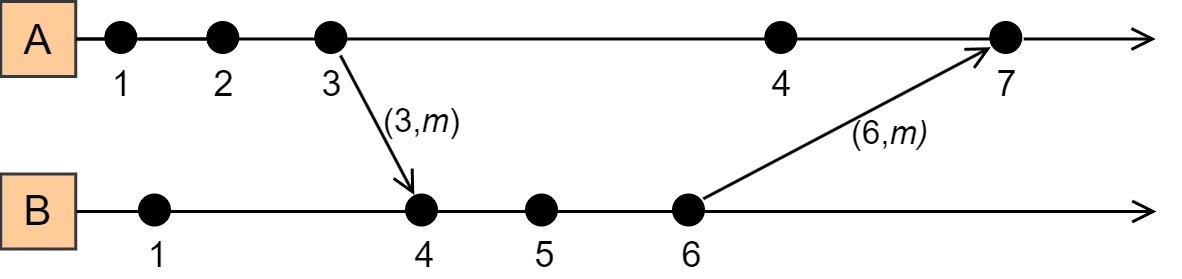
\includegraphics[width=10cm]{LamportClocks.jpg}
    \caption{Example of lamport clocks. \textit{m} represents a message.}
    \label{fig:lamport}
\end{figure}

Lamport clocks give us the following guarantee, where $L(a)$ is the lamport timestamp of event $a$: 
\begin{itemize}
    \item $a \rightarrow b \implies  L(a) < L(b)$
\end{itemize}
This is useful for detecting potential causal dependencies. However, by using lamport clocks, concurrent events may appear to be causally dependent. One use for lamport clocks is to create a total order ($\prec$) which captures the causal dependencies. This can be achieved by assigning each node a unique ID, and using that to break ties when $L(a) = L(b)$. When an event happens on a node, the node ID is then also stored in the lamport timestamp. It is worth noting that this total order is arbitrary, but deterministic. This was defined by Lamport\cite{lamport1978time}, and can be denoted as:\par
\[a \prec b \iff L(a) < L(b) \lor (L(a) = L(b) \land ID(a) < ID(b))\]

\subsection{Vector Clocks}
Vector clocks are another logical clock that provide more gurantees than lamport clocks. Each node maintains a vector timestamp, which is a vector of counters. Each counter corresponds to a node in the system.
When an event occurs on a node, the node increments its own counter in the vector and sends the updated vector to the other nodes.
When a node receives a timestamp, it updates its own vector timestamp to be the maximum of the two timestamps. \cite{mattern1989virtual}.\par

Vector timestamps can be ordered by the following rules, where $V(a)$ is the timestamp of event $a$ and $V(a)_i$ is the value of the counter for node $i$:
\[V(a) \leq V(b) \iff \forall_i [V(a)_i \leq V(b)_i]  \]
\[V(a) = V(b) \iff \forall_i [V(a)_i = V(b)_i]\]

Lamport clocks can only indicate \emph{potential} causal dependencies. Vector timestamps are larger than Lamport timestamps, but they precisely indicate the happened-before relation between events in a system. This is denoted by the following ($\vert \vert$ denotes concurrent):

\begin{itemize}
    \item $a \rightarrow b \iff V(a) \leq V(b) \land V(a) \not = V(b)$
    \item $a = b \iff V(a) = V(b)$
    \item $a \: || \:  b \iff V(a) \not \leq V(b) \land V(b) \not \leq V(a)$
\end{itemize}

This can be used to create a partial order, as concurrent events are neither causally related nor ordered with respect to each other.

\begin{figure}
    \centering
    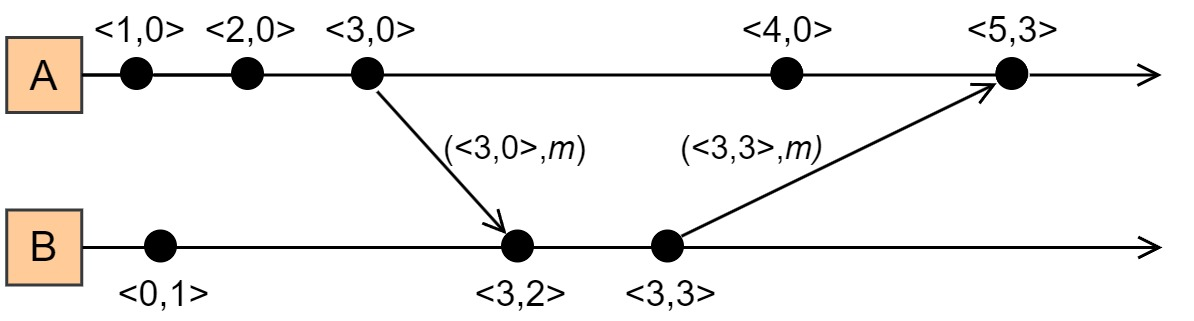
\includegraphics[width=10cm]{VectorClocks.jpg}
    \caption{Example of vector clocks. The first and second values correspond to nodes A and B respectively. \textit{m} represents a message.}
    \label{fig:vector}
\end{figure}

\section{Conflict-free Replicated Data Types}
Conflict-free Replicated Data Types (CRDTs) are types of data structures, such as sets, counters, and registers, that can be replicated across multiple nodes in a distributed system. They are unique in that the data type itself is responsible for resolving conflicts, rather than the application. 

CRDTs were created to allow for a better eventually consistent model, that can increase availability and performance while removing the need for conflict arbitration.  One main factor that allows CRDTs to guarantee SEC is that the data types are commutative\cite{10.1007/978-3-642-24550-3_29}, meaning that the updates can be applied in any order. Although, certain CRDTs may rely on causal consistency to operate correclty. They also do not require a main or primary elected server, as each node can resolve the conflicts by themselves. Therefore, CRDTs are applicable in a peer-to-peer environment. \par
One useful application for CRDTs is their ability for offline use \cite{10.1145/3359591.3359737}. If an application is built using CRDTs, it can feel more responsive as updates to the state can be made locally without the system having to wait on replies from remote servers. \par
There are two main types of CRDTs, state-based and operation-based. Both have different ways of sending updates to other nodes, and different ways of resolving conflicts. \par


\subsection{State-Based (CvRDTs)}

\begin{figure}
    \centering
    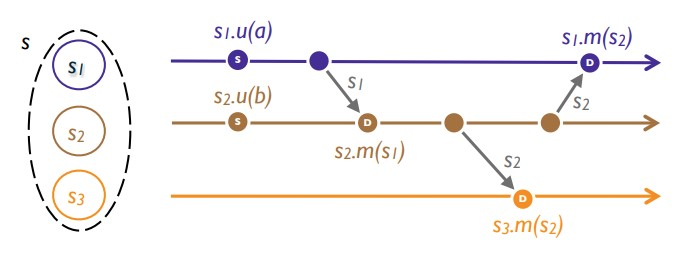
\includegraphics[width=8cm]{state.jpg}
    \caption{State-based CRDT replication. Reproduced from \cite{10.1007/978-3-642-24550-3_29}}
    \label{fig:statebased}
\end{figure}

State-based CRDTs, or otherwise called Convergent Replicated Data Types (CvRDTs), send their full state to other replicas where they are merged by a function to form a new state. The \textit{merge} function must be associative, commutative and idempotent \cite{10.1007/978-3-642-24550-3_29}. As the state of a CvRDT grows in size, the entire state must be sent, which can result in high bandwidth usage. However, since CvRDTs send their full state, missed updates do not break the system because the next state transmission includes all previously missed updates. As a result, there are fewer requirements on the replication layer. Also, CvRDTs can make use of gossip protocols (as shown in Figure \ref{fig:statebased}) which helps reduce network usage. \par

Delta State CRDTs are a form of state-based CRDTs that only send the changed, or the delta, part of the state. This allows for the messages sent between replicas to be smaller and work across unreliable networks \cite{Almeida_2018}. They, therefore, have the best of both operation and state-based CRDTs.


\subsection{Operation-Based (CmRDTs)}

\begin{figure}
    \centering
    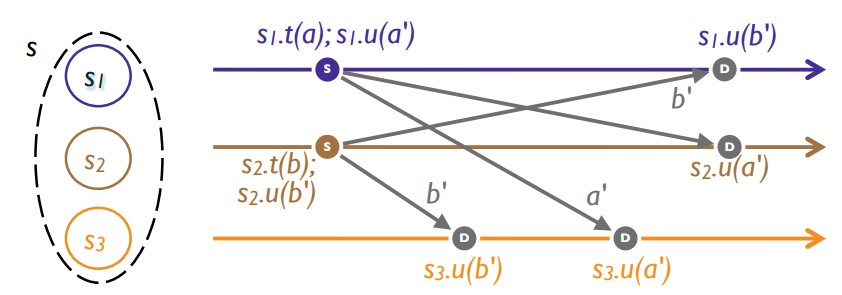
\includegraphics[width=8 cm]{operation.jpg}
    \caption{Operation-based CRDT replication. Reproduced from \cite{10.1007/978-3-642-24550-3_29}}
    \label{fig:operation}
\end{figure}

Operation-based CRDTs, or otherwise called Commutative Replicated Data Types (CmRDTs), only send operations to other replicas. Each update to the data is a pair consisting of a \textit{prepare} method and an \textit{effect} method. The \textit{prepare} method is executed at the local replica and produces a message representing the operation, and the \textit{effect} method applies this operation to the state\cite{10.1007/978-3-642-24550-3_29}. The operations have to be commutative, but not idempotent. As CmRDTs only send operations, each replica must receive all operations otherwise the state will be incorrect. Therefore, there are more requirements on the replication layer. Figure \ref{fig:operation} shows an example of this replication. \par

\textit{Pure} operation-based CRDTs were proposed to create better operation-based CRDTs\cite{10.1007/978-3-662-43352-2_11}. These impose restrictions on the \textit{prepare} method, requiring that it does not inspect the current state and can only return the operation. Additionally, the state of the object is composed of a partially ordered log of operations. It is possible to reduce the state size by implementing a method that strips causality information from operations once they become \textit{"causally stable"}\cite{10.1007/978-3-662-43352-2_11}.

It is important to note that operation-based CRDTs are more applicable to \textit{static} distributed systems, where the number of replicas is fixed. Papers about operation-based CRDTs usually assume a fixed number of replicas, such as \cite{baquero2017pure}. There are ways to make operation-based CRDTs work well in \textit{dynamic} systems, such as using dotted version vectors \cite{preguiça2010dotted}. For the remainder of this paper, the terms 'static' and 'dynamic' systems will be used as defined above. The focus of this paper will be on static systems, as dynamic systems are beyond its scope.\par 

It is important to note that operation-based CRDTs usually require reliable causal broadcast \cite{10.1007/978-3-662-43352-2_11}, which can be complex. However, for the purpose of this paper, a rudimentary reliable causal broadcast algorithm will be implemented. If the CRDTs discussed in this paper are to be used in a real-world application, a more complex reliable causal broadcast algorithm should be used \cite{10.1145/128738.128742}. \par

\subsection{CRDTs and File Systems}
A file system can be represented as a tree structure, where the files and directories are the nodes and the directory hierarchy is represented by the branches between nodes. Therefore, a tree CRDT can be used to create a distributed/replicated file system that will have high availability and low latency. Tree-structured CRDTs have been created before \cite{10.1145/2757667.2757683}, \cite{kleppmann2018automerge}. However, designing a tree CRDT with a \textit{highly available} (or \textit{atomic}) move operation poses significant challenges due to the need to preserve the strict tree invariant. \textit{Highly available} meaning: does not require locking, consensus and does not create duplicates.   \par

This can be shown by ElmerFS (A file system created using CRDTs), where concurrent moves can create a cycle \cite{10.1145/3465332.3470872}. Najafadeh et al. \cite{Najafzadeh0E18} proposes a similar system which instead locks on move operations to ensure cycles are not created. These papers show how hard creating a highly available move operation is, however recent work has shown that it is possible \cite{9563274}, \cite{https://doi.org/10.48550/arxiv.2103.04828}, \cite{https://doi.org/10.48550/arxiv.1805.04263}. \par

\subsection{Move Operations in Tree CRDTs}
Tree CRDTs themselves are not difficult to implement, as shown by the paper "Abstract unordered and ordered trees CRDT" \cite{martin2012abstract} from 2012. Tree CRDTs have also been using in real-time collaborative editing applications \cite{5158449}. However, these implementations only allow for adding and removing nodes, not moving them. This is because a highly available move operation is difficult to implement, as concurrent moves can break the tree invariant. Therefore, this section will exclusively consider conflicts that arise from move operations, as these represent new advancements in tree CRDTs. 

There are three main operations that will need to be considered when implementing conflict resolution. These being: \textit{add(p,n)}, \textit{remove(n)} and \textit{move(p,n)}. Where \textit{p} is the parent node, and \textit{n} is the globally unique id of the node to be added, removed or moved. $Add$ will add node \textit{n} under parent node \textit{p}, $remove$ will remove node \textit{n} and $move$ will move node \textit{n} to parent node \textit{p}. Considering these operations, the following describes the conflicts that can arise from concurrent operations involving move operations:

\addtocounter{footnote}{1}

\begin{itemize}
    \item
        \textit{Move-Add} conflict - This conflict has one case: 
        \begin{itemize}
            \item The move operation moves node $n_1$ with name $m$ is under node $p$, while the add operation adds node $n_2$ with name $m$ under node $p$\footnotemark[\value{footnote}]
        \end{itemize}
    \item
        \textit{Move-Remove} conflict - This conflict has two cases:
        \begin{itemize}
            \item 
                The move operation moves node $n$ under node $p$, while the remove operation removes node $p$
            \item
                The move operation moves node $n$ under node $p$, while the remove operation removes node $n$
        \end{itemize}
    \item
        \textit{Move-Move} conflict - This conflict has three cases:
        \begin{itemize}
            \item One move operation moves node $n_1$ with name $m$ under node $p$, while the other move operation moves node $n_2$ with name $m$ under node $p$\footnotemark[\value{footnote}]
            \item Two move operations move the same node $n$ to different parents $p_1$ and $p_2$
            \item One move operation moves node $n_1$ under node $n_2$, while the other move operation moves node $n_2$ under node $n_1$, creating a cycle
        \end{itemize}
\end{itemize}

\footnotetext[\value{footnote}]{This conflict will only arise if nodes are uniquely identified by their name and parent, as is typical in file systems. (However, for other systems this may not be the case)}

The conflict resolution will not be discussed here, as it will be a part of the algorithms discussed in the next section. Each algorithm will have its own conflict resolution strategy. It is important to note that the algorithms, as they are, do not uniquely identify nodes by their name and parent. And therefore, do not resolve those conflicts. These algorithms may be adapted to resolve these conflicts, and if time permits, this paper will explore such modifications.


\subsection{Algorithms With a Highly Available Move} \label{sssec:algorithms}
Currently, there two main proposed algorithms that allow a highly available move operation. It must be noted that Najafzadeh et al. \cite{Najafzadeh0E18} has shown that any coordination-free solution will have anomalies, such as having to ignore certain operations. The following section will discuss these algorithms and how they work: \par
\begin{itemize}
    \item
          \textbf{Kleppmann et al. \cite{9563274}} proposes an algorithm based off previous work by Kleppmann, called OpSets \cite{https://doi.org/10.48550/arxiv.1805.04263}. The general approach is to have a total order for all operations, which can be achieved using lamport timestamps. Along with \textit{undo} and \textit{redo} operations. Using these, the algorithm will apply each operation in the correct order, undoing and redoing operations as necessary. A \textit{log} is required to store all previous operations so that the algorithm can undo and redo operations. There is only one correct way for the operations to be applied and therefore one final state. An operation is ignored if it would cause an invalid tree state (a cycle), or if the node or new parent does not exist. It is possible to trim the log to reduce the amount of memory required using a causally stable threshold, however this will not be discussed here. \par
          \begin{itemize}
            \item This algorithm has the overhead of having to undo and redo operations, however, it is easily extensible to add other conflicts (such as file name conflicts). \par
            \item Operations can be applied immediately, as if they are dependent on any other operation, they will eventually be applied in the correct order. \par
            \item This algorithm may produce unwanted behaviour, as it uses lamport timestamps to order operations. This means that if two operations are performed concurrently, the order they are applied is arbitrary (but deterministic). \par
          \end{itemize}

          \begin{figure}
            \centering
            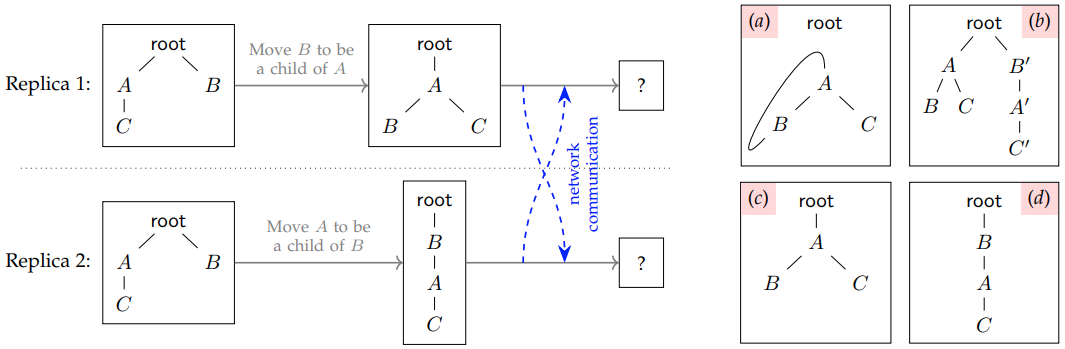
\includegraphics[width=1\textwidth]{kleppmann.png}
            \caption{Concurrent move operations causing a cycle. Kleppmann's algorithm prefers the move from the replica with the lower ID and ignores the other operation (producing \textit{c} in this case). Reproduced from \cite{9563274}}
            \label{fig:kleppmann}
        \end{figure}
          
        %   represents the tree as a set of parent-child relationships. A move operation is performed by removing the node from wherever it is in the tree and moving it to its new location. This operation can also be used for adding and removing nodes, the former by creating a new node under the specified parent and the latter by moving the node under a "trash" node. It stores a \textit{log} of all previous operations, which allows the algorithm to implement a move operation. The algorithm can use the \textit{log} to ensure that all operations are applied in the correct order by undoing and reapplying operations (as proposed in \cite{https://doi.org/10.48550/arxiv.1805.04263}). It deals with cycles by ensuring that if any operations were to create a cycle, it would be ignored however they are still added to the \textit{log}. In general, the algorithm will prefer the latest operation that does not cause a conflict. The only conflict which the algorithm does not resolve is child nodes with the same parent having the same name.

    \item
          \textbf{Nair et al. \cite{https://doi.org/10.48550/arxiv.2103.04828}} proposes \textit{Maram}, a "light-weight" tree CRDT algorithm. It only applies conflict resolution for concurrent move operations. The paper defines two types of move operations, \textit{up-moves} and \textit{down-moves}. An \textit{up-move} is a move operation that moves a node towards the root, or to the same distance from the root. A \textit{down-move} is a move operation that moves a node away from the root. Each move operation also has a priority. The idea is, that concurrent up-moves are safe (as they do not cause a cycle), and therefore do not need conflict resolution. Whereas, two concurrent down-moves, or an up-move and a down-move require conflict resolution if both operations move a node into the critical descendants (as shown in Figure \ref{fig:maram}) of the other move operation. In the case of a concurrent up-move and down-move, the up-move wins. In the case of concurrent down-moves, the move with the highest priority wins. The priority is a unique number that is assigned to each move operation.
          \begin{itemize}
            \item This algorithm has the overhead of having to resolve conflicts for concurrent move operations, but not for any other operations. \par
            \item It requires a priority to be assigned to each move operation, which may be difficult to implement in some systems. \par
            \item It has more overhead for timestamps, as the timestamps must be able to detect concurrent operations. \par
            \item It is harder to extend to other types of conflicts, such as file name conflicts, as its conflict resolution policy is specific to move operations that cause cycles. \par
          \end{itemize}
          

\begin{figure}[H]
    \centering
    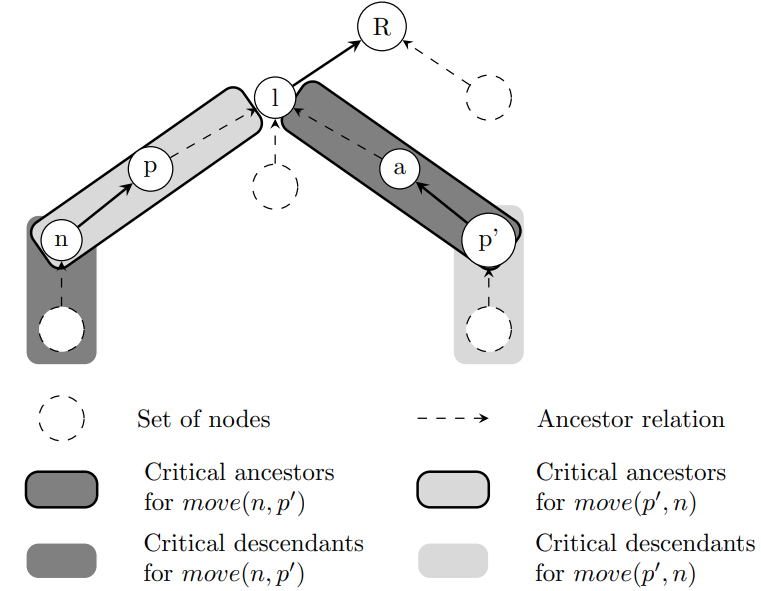
\includegraphics[width=0.6\textwidth]{maram.png}
    \caption{Critical ancestors and critical descendants for concurrent move operations, \textit{move(node, newparent)}. \textit{l} is the closest common ancestor. Reproduced from \cite{https://doi.org/10.48550/arxiv.2103.04828}.}
    \label{fig:maram}
\end{figure}

\end{itemize}

These will be referred to as \textit{Kleppmann's algorithm} and \textit{Maram} respectively, and will be the main focus of this paper.

Table \ref{table:differences} shows a comparison between the two algorithms:

\begin{table}[h]
    \def\arraystretch{2}
    \caption{Comparison of Algorithms} % title of Table
    \centering % used for centering table
    \begin{tabular}{c c c} % centered columns (4 columns)
        \hline\hline %inserts double horizontal lines
                                & \textbf{Kleppmann's \cite{9563274}} & \textbf{Nair's (\textit{Maram}) \cite{https://doi.org/10.48550/arxiv.2103.04828}} \\ [0.5ex] % inserts table
        %heading
        \hline % inserts single horizontal line
        \textbf{Delivery Layer} & \makecell{Eventual Consistency                                                                                          \\ \textit{Low Cost}} & \makecell{Causal Consistency\textsuperscript{i}  \\ \textit{Higher Cost}}  \\ % inserting body of the table
        \textbf{Operation Order}     & \makecell{Total Order                                                                                                   \\ \textit{High Cost}} & \makecell{Partial Order \\ \textit{Low Cost}}

        \\ [1ex] % [1ex] adds vertical space
        \hline %inserts single line
    \end{tabular}
    \label{table:differences} % is used to refer this table in the text
\end{table}

\textsuperscript{i}\textit{Causal Consistency} gurantees that if two operations are causally related, then the second operation will be applied after the first operation on all replicas. For example, if a replica receives operation \textit{A} then creates operation \textit{B}, then operation \textit{A} should be applied before operation \textit{B} on all other replicas. \par

\begin{figure}[H]
    \centering
    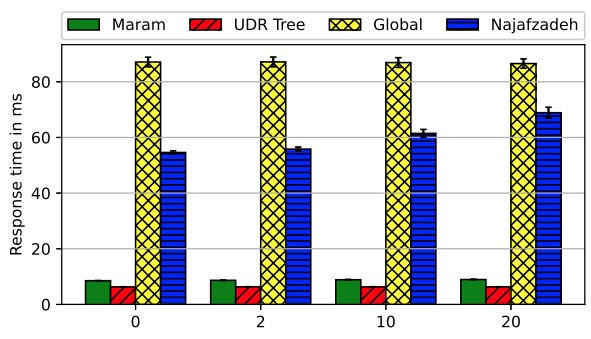
\includegraphics[width=10cm]{Response.jpg}
    \caption{Response time for different conflict rates (0-20\%). Reproduced from \cite{https://doi.org/10.48550/arxiv.2103.04828}}
    \label{fig:responsetime}
\end{figure}

Figure \ref{fig:responsetime} shows differences in response times between different algorithms. Kleppmann's algorithm \cite{9563274} can be regarded as a UDR Tree, and therefore we can see that it has a slightly lower response time than Maram \cite{https://doi.org/10.48550/arxiv.2103.04828}. Figure \ref{fig:responsetime} also shows how a lower response time can be achieved by using non-locking algorithms.


This paper will use both of the algorithms stated above, Kleppmann's \cite{9563274} and Nair's (\textit{Maram}) \cite{https://doi.org/10.48550/arxiv.2103.04828}. The implementation of these algorithms, and subsequent testing, will be the main part of this project. The testing will inform the evaluation, which will compare the two algorithms and determine their viability. Notably, these algorithms require a separate delivery layer to communicate between replicas. This layer will be implemented separately from the CRDTs.


\newpage
\chapter{Planning}
The original aim of this paper was to create a file synchronisation system using conflict-free replicated data types (CRDTs). However, due to the complexity and challenges of implementing such a system, this paper has narrowed its focus to explore the implementation and evaluation of the CRDTs. By narrowing down the scope of this research, this paper aims to provide a more in-depth analysis of the advantages and limitations of the CRDTs. This will allow for a more thorough evaluation of the CRDTs, and will allow for a more detailed comparison between the different CRDTs.

\section{Requirements}
The main focus of this paper is to implement the two CRDT algorithms, \cite{9563274} and \cite{https://doi.org/10.48550/arxiv.2103.04828}, and to test them individually as well as to compare them. While the evaluation of these algorithms will be the main focus, this paper will also attempt to create implementations that can be used by other developers. As such, the requirements will be as follows:
\begin{itemize}
    \item The system shall be comprised of multiple layers that can be modified independently.
    \item The system should have a simple and easy to use API.
    \item The implementations should follow the literature as closely as possible, to ensure they are logically correct.
    \item The system shall support immediate local execution of operations on the CRDTs.
    \item The replication between replicas shall be handled by a separate layer than that which handles the CRDTs. This will allow for the replication layer to be modified independently of the CRDT layer, and vice versa.
    \item The replication layer should handle the communication between a fixed number of replicas asynchronously.
    \item Each layer should have an interface that allows for other implementations to be created and swapped in. This will allow for the system to be easily modified and extended.
\end{itemize}


\section{System Architecture}\label{sec:architecture}

The design will be split into different layers that will each be independent and can be modified separately. The layers are as follows:
\begin{itemize}
    \item \textbf{CRDT} This layer will be in charge of conflict resolution and is the main focus of this paper. The CRDTs will be implemented using the algorithms described in Section \ref{sssec:algorithms}. This layer is responsible for the following: 
        \begin{itemize}
            \item Applying operations (which will be \textit{local} or \textit{remote}) on the CRDT
            \item Resolving conflicts that arise between concurrent operations 
            \item Ensuring that all replicas eventually converge to the same state, if they have all received the same operations
            \item Keeping track of the state of the CRDT (the state of the tree)
            \item Providing an interface for application code to interact with the CRDT
        \end{itemize}

    \item \textbf{Interface} This layer will provide a uniform interface to the user, as well as provide the connection between the CRDT and Network layer. It will need to be able to:
        \begin{itemize}
            \item Ensure that operations are applied to the local CRDT only when they are ready to be applied (This will depend on the chosen consistency model)
            \item Buffer operations that are not ready to be applied on the local CRDT
            \item Provide an interface for application code to interact with the CRDT
            \item Ensure that all operations are sent to the network layer for replication
        \end{itemize}
    \item \textbf{Network} This layer will be in charge of network communications. It will need to be able to:
        \begin{itemize}
            \item Connect to other peers, and share peers with other peers
            \item Send and Receive operations to and from other peers
            \item Ensure that operations are sent to all peers, even if some peers are offline
            \item Buffer operations to be sent to peers that are offline
        \end{itemize}
\end{itemize}
Certain CRDTs require different consistency models, therefore the interface layer will ensure that incoming operations are applied correctly. It is important that each CRDT is correctly paired with the correct consistency model, as otherwise the CRDT may not work correctly. \par

\section{Language and Tools}
\subsection{Go}
Go is a language created by Google, and is designed to be used in distributed systems with the help of its built-in, lightweight concurrency features. As this paper aims to create a distributed system, then Go is a good choice to help with this. \par

The CRDTs which will be implemented by this paper are particularly applicable to distributed file systems. Recent distributed file systems have been written using Go, such as JuiceFS or Kertish-DFS. Therefore, by using Go this paper aims to create useful implementations for these systems, or to provide a base implementation which can then be improved upon. \par


\subsection{GitHub}
The source code for this project will be stored in a GitHub repository. This will allow for the code to be easily shared and modified by other developers. It will also allow for the code to be easily version controlled, and for the history of the project to be easily tracked. This report is also stored in the GitHub repository. \par

\subsection{Diagrams}
LucidChart\footnote{https://www.lucidchart.com/} is an online tool which can be used to create different types of diagrams. This paper will use LucidChart to create UML class diagrams, which will be used to visualise the different components of the system. Eraser\footnote{https://www.eraser.io} is another online tool which can be used to create diagrams from code. This paper will use Eraser to create sequence diagrams, which will be used to visualise the flow of the system. \par


\section{Testing}
Go has a built-in testing framework, which will be used to test the code. Unit tests can be used to simulate concurrent operations on the CRDTs, and therefore test the correctness of the CRDTs. Integration tests will be used to test the correctness of the system as a whole and ensure that the different layers work together correctly. \par


\section{Code Structure}\label{sec:code_structure}
The code will be written in accordance with the Go style guide\footnote{https://golang.org/doc/effective\_go}. This will ensure that the code is easy to read and understand. Go itself is opinionated about how code should be structured, and comes with a built-in tool to automatically format code. This makes code written in Go consistent and easy to read. \par

The code will be split into different packages, with each package containing a single component of the system. The packages will be as follows:
\begin{itemize}
    \item \textbf{TreeCRDT} This package will contain the implementations of the CRDTs. This package will be the main focus of this paper, and will contain the implementations of the two CRDTs described in Section \ref{sssec:algorithms}. However, usually this package should not be used directly, as it does not provide an interface for application code to interact with the CRDTs. Instead, the \textbf{Interface} package should be used. 
    \item \textbf{TreeInterface} This package will contain the interface for application code to interact with the CRDTs, as well as the connection between the CRDTs and the Network layer.
    \item \textbf{Connection} This package will contain a generic interface for the Interface layer to interact with the Network layer. It will contain the classes that will handle reliable communication between replicas.
    \item \textbf{Clocks} This package will contain the implementations of the clocks and timestamps.
\end{itemize}

\newpage
\chapter{Design}
The system will be designed according to Section \ref{sec:architecture}. The design will attempt to use interfaces where possible, to allow for the system to be easily modified and extended. 

\section{Package Structure}
The system will be split into different packages as described in Section \ref{sec:code_structure}. The \texttt{TreeCRDT} package is the CRDT layer. The \texttt{TreeInterface} is the Interface layer. And the \texttt{Connection} package is the Network layer. The dependencies between these packages are shown in Figure \ref{fig:packages}.

\begin{figure}[H] 
    \centering
    \fbox{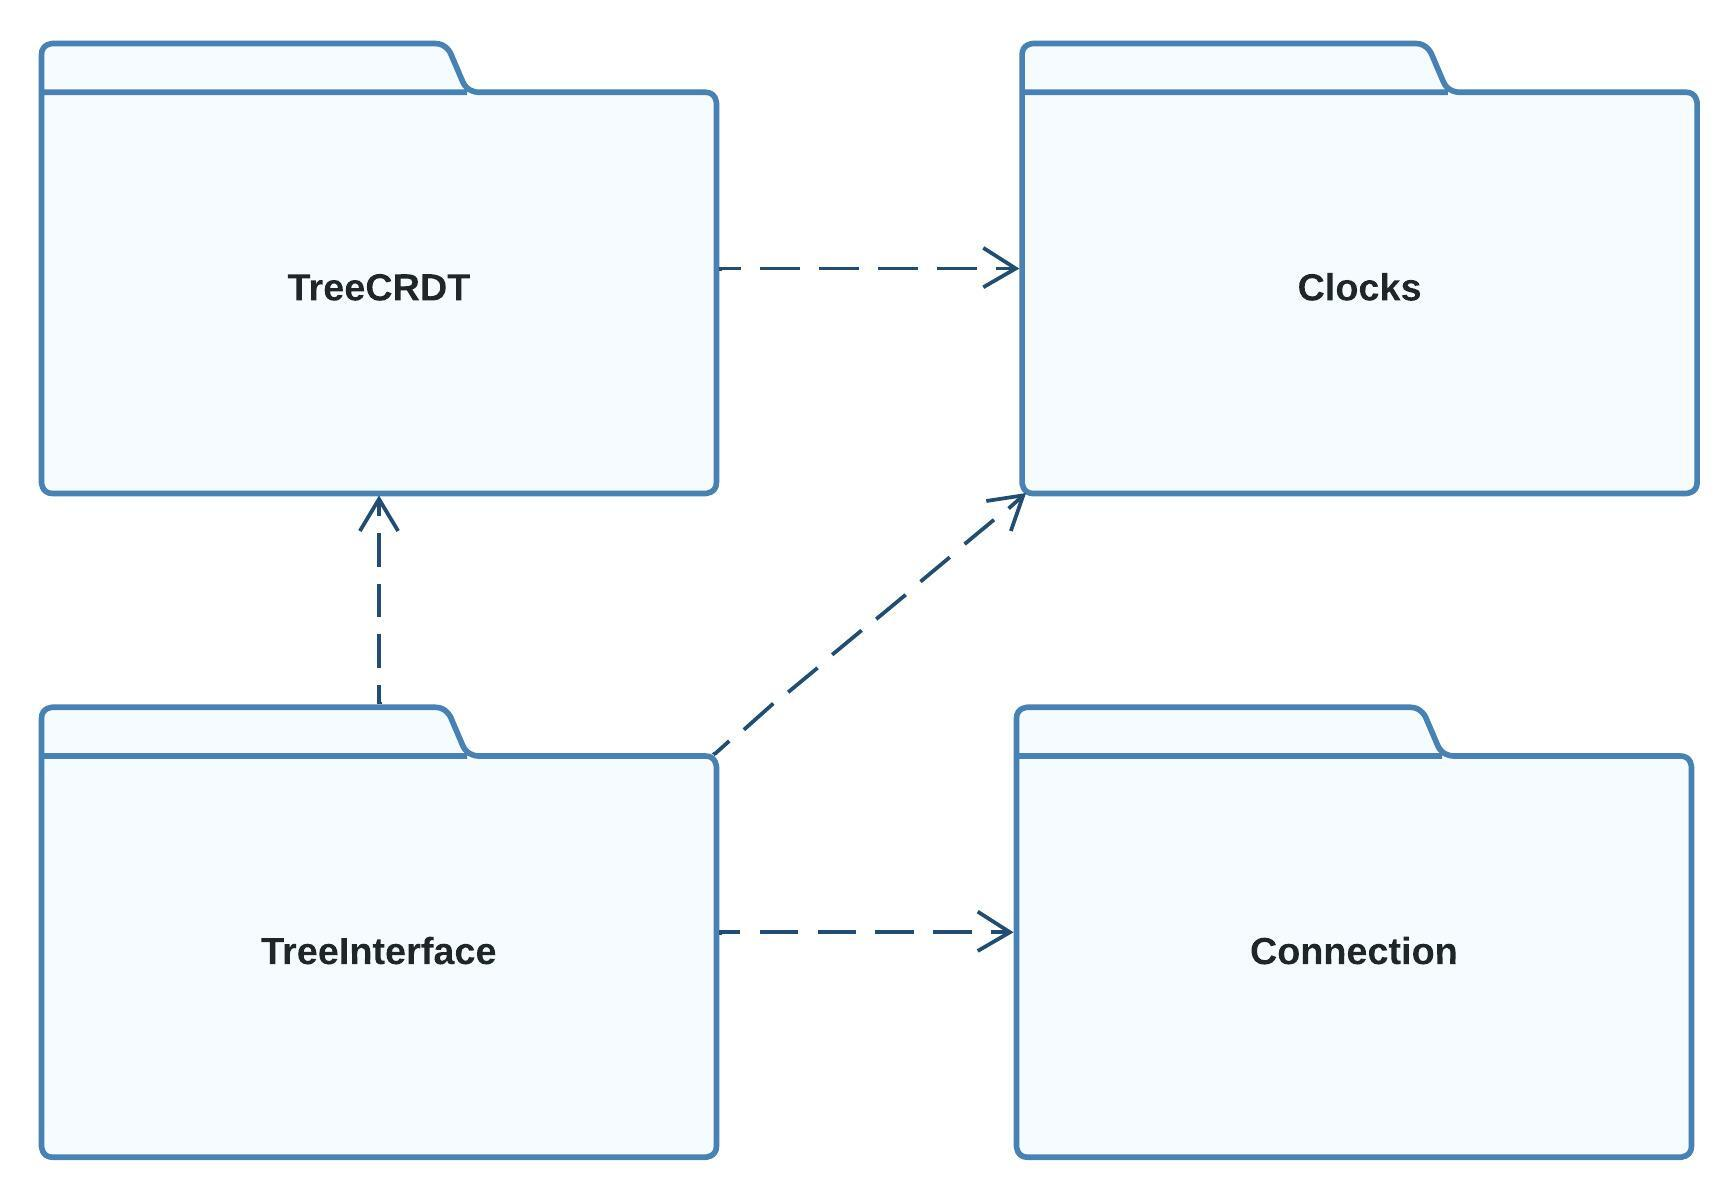
\includegraphics[width=12cm]{packages.jpeg}}
    \caption{Package structure for the project, with dependencies shown.}
    \label{fig:packages}
\end{figure}

The packages will be developed in a way which implements the main focus of this paper first, the CRDTs. Therefore, they will be developed in the following order: \texttt{Clocks}, \texttt{TreeCRDT}, \texttt{Connection} and finally \texttt{TreeInterface}. This will allow for the main focus of this paper to be implemented first, and then the rest of the system can be built around it. \par

\section{System Structure}

\subsection{Clocks}
The system has two interfaces for tracking the order of events, clocks and timestamps. Moving forward, \textit{clocks} will refer to a timestamp for a specific actor, and \textit{timestamps} will refer to a timestamp for a specific event.  
As shown in Figure \ref{fig:ordered}, the system will have two implementations of clocks, Lamport and Vector clocks. These will be used within their respective CRDTs, as described in Section \ref{sssec:algorithms}. \par

\begin{figure}[h]
    \centering
    \fbox{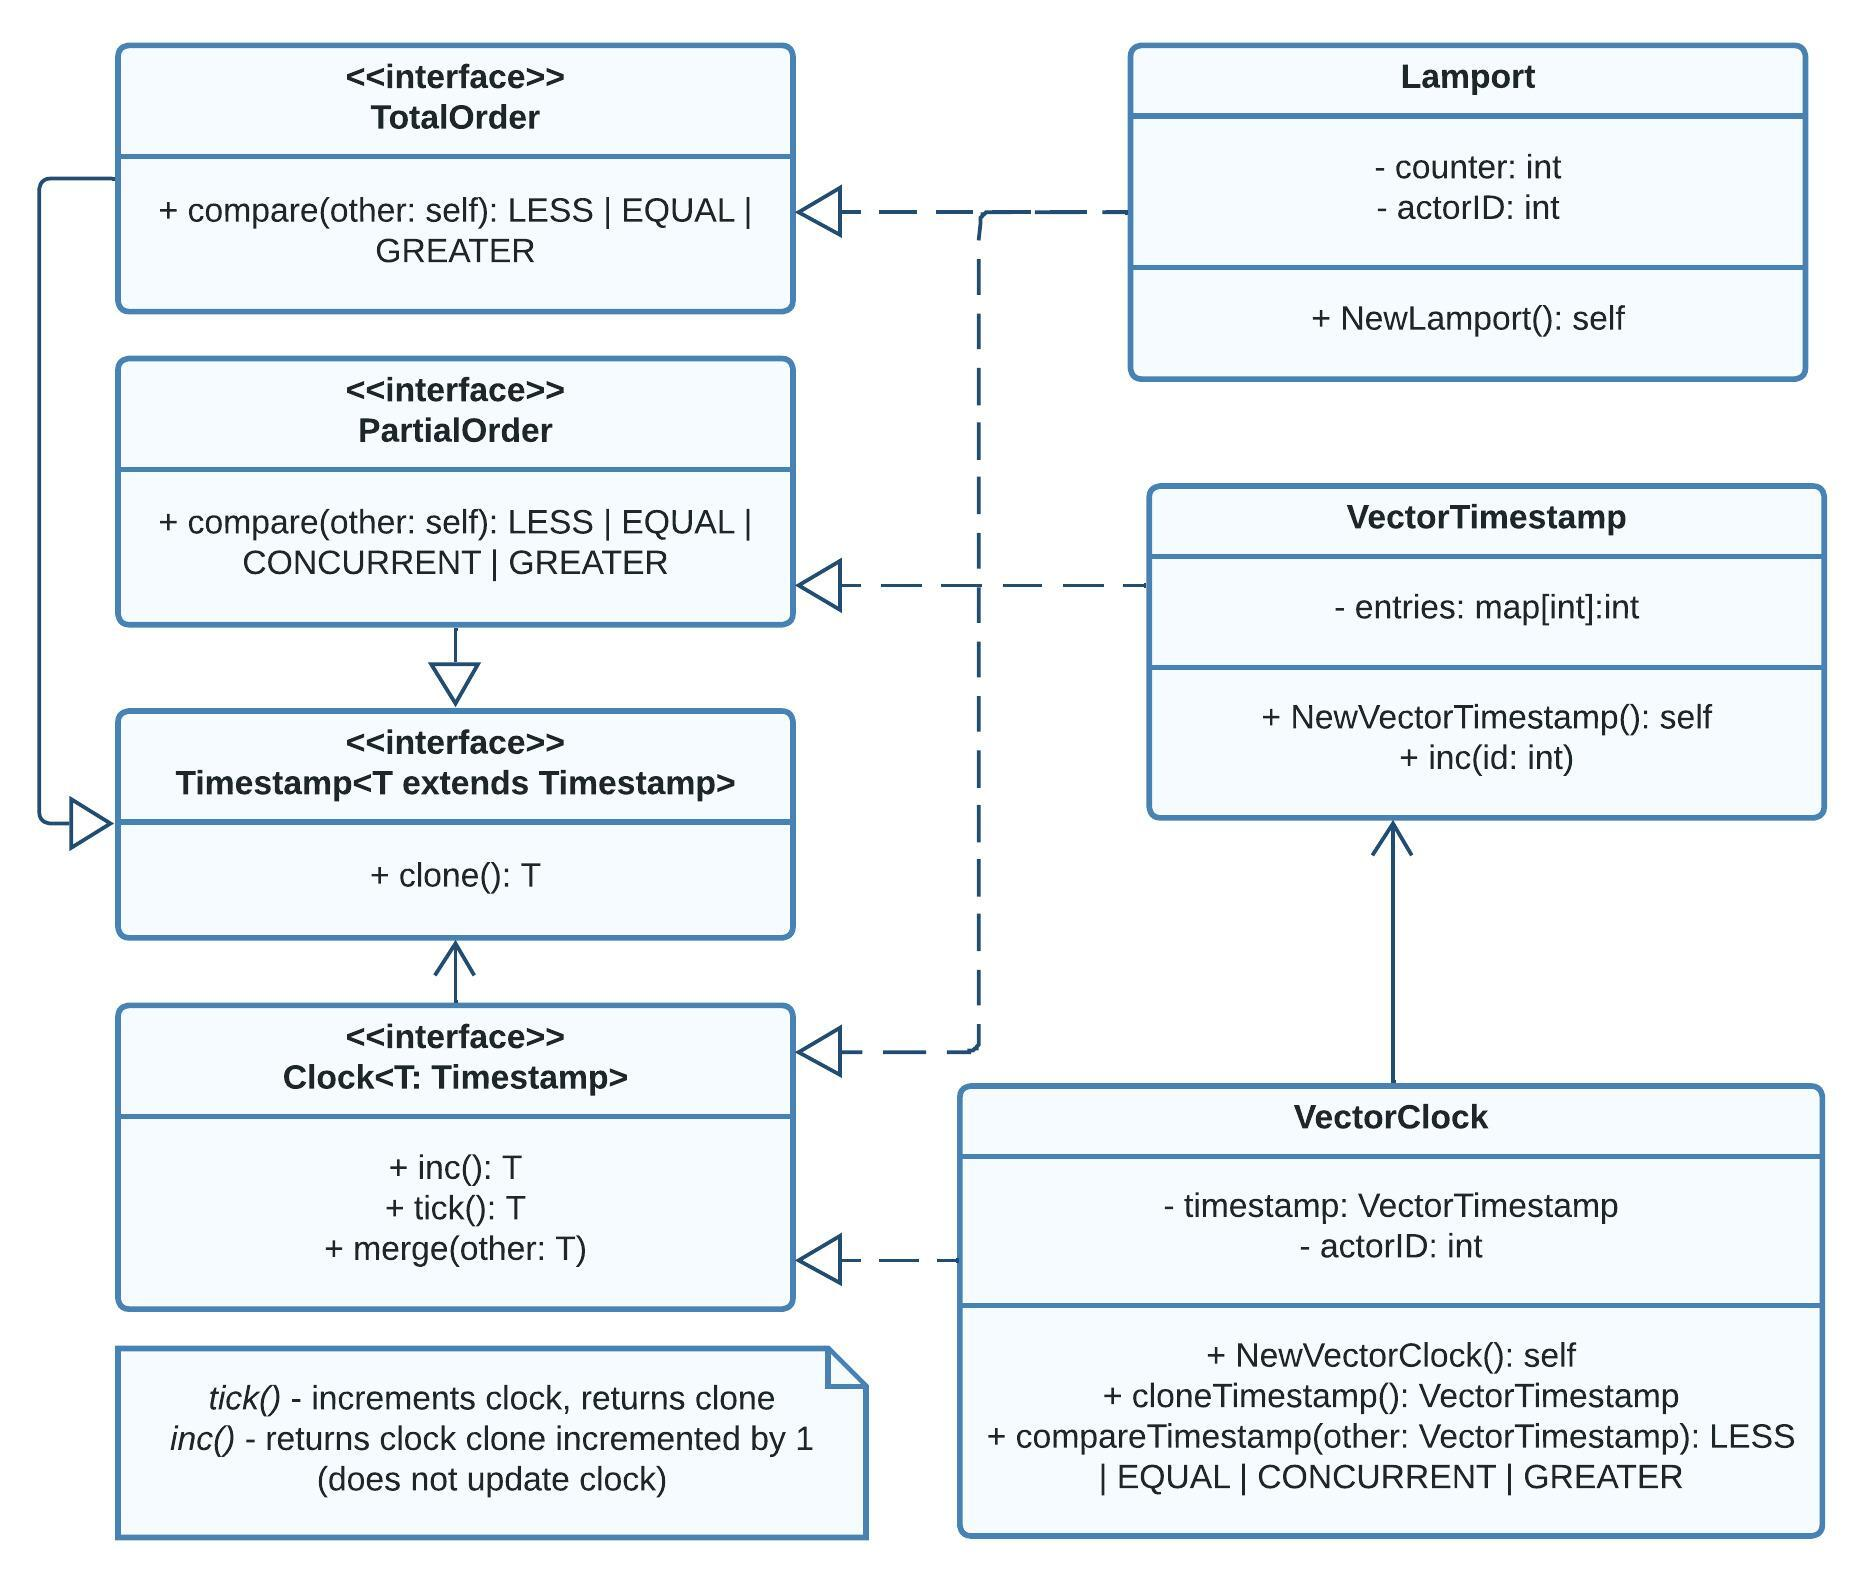
\includegraphics[width=13cm]{clocks.jpeg}}
    \caption{Class diagram for the clocks and timestamps. Including Lamport and Vector clocks.}
    \label{fig:ordered}
\end{figure} 

The two interfaces, \texttt{Clock} and \texttt{Timestamp}, are shown in Figure \ref{fig:ordered}. The class \texttt{Lamport} implements both, as it is both a timestamp and a clock. The Vector clock is split into two classes, \texttt{VectorClock} and \texttt{VectorTimestamp}. The \texttt{VectorClock} implements the \texttt{Clock} interface, and the \texttt{VectorTimestamp} implements the \texttt{Timestamp} interface. \par

The \texttt{Lamport} and \texttt{VectorTimestamp} classes implement \texttt{TotalOrder} and \texttt{PartialOrder} respectively. They denote the differences in the gurantees that the two types of clocks provide. The \texttt{Lamport} class implements \texttt{TotalOrder} as it provides an arbitrary, but deterministic total order of events. The \texttt{VectorTimestamp} class implements \texttt{PartialOrder} as it provides a partial order of events. \par

\subsection{CRDT and Interface}
Since the CRDT layer is the primary focus of this paper, it will comprise multiple components, making it the largest layer. The components will be specific to each CRDT, and will be implemented using the algorithms described in Section \ref{sssec:algorithms}. The exact implementation is not known at this point, and will be discussed in Section \ref{sec:implementation}. \par


The exact \texttt{Components} of each CRDT will be known once the algorithms have been implemented. It may also be possible to provide a \texttt{CmRDT} interface for the CRDTs, with \textit{prepare} and \textit{effect} methods. However, this will not be explored in this paper. \par

The classes that implement \texttt{Tree} from Figure \ref{fig:crdt} will also be responsible for sending operations to the network layer to be broadcast to other peers. As well as receiving operations from the network layer, and either applying them to the local CRDT or buffering them, depending on the consistency model. They will also be responsible for providing a generic interface for application code to interact with the CRDT, and translating the application code into operations for the specific CRDT. \par

\begin{figure}[H]
    \centering
    \fbox{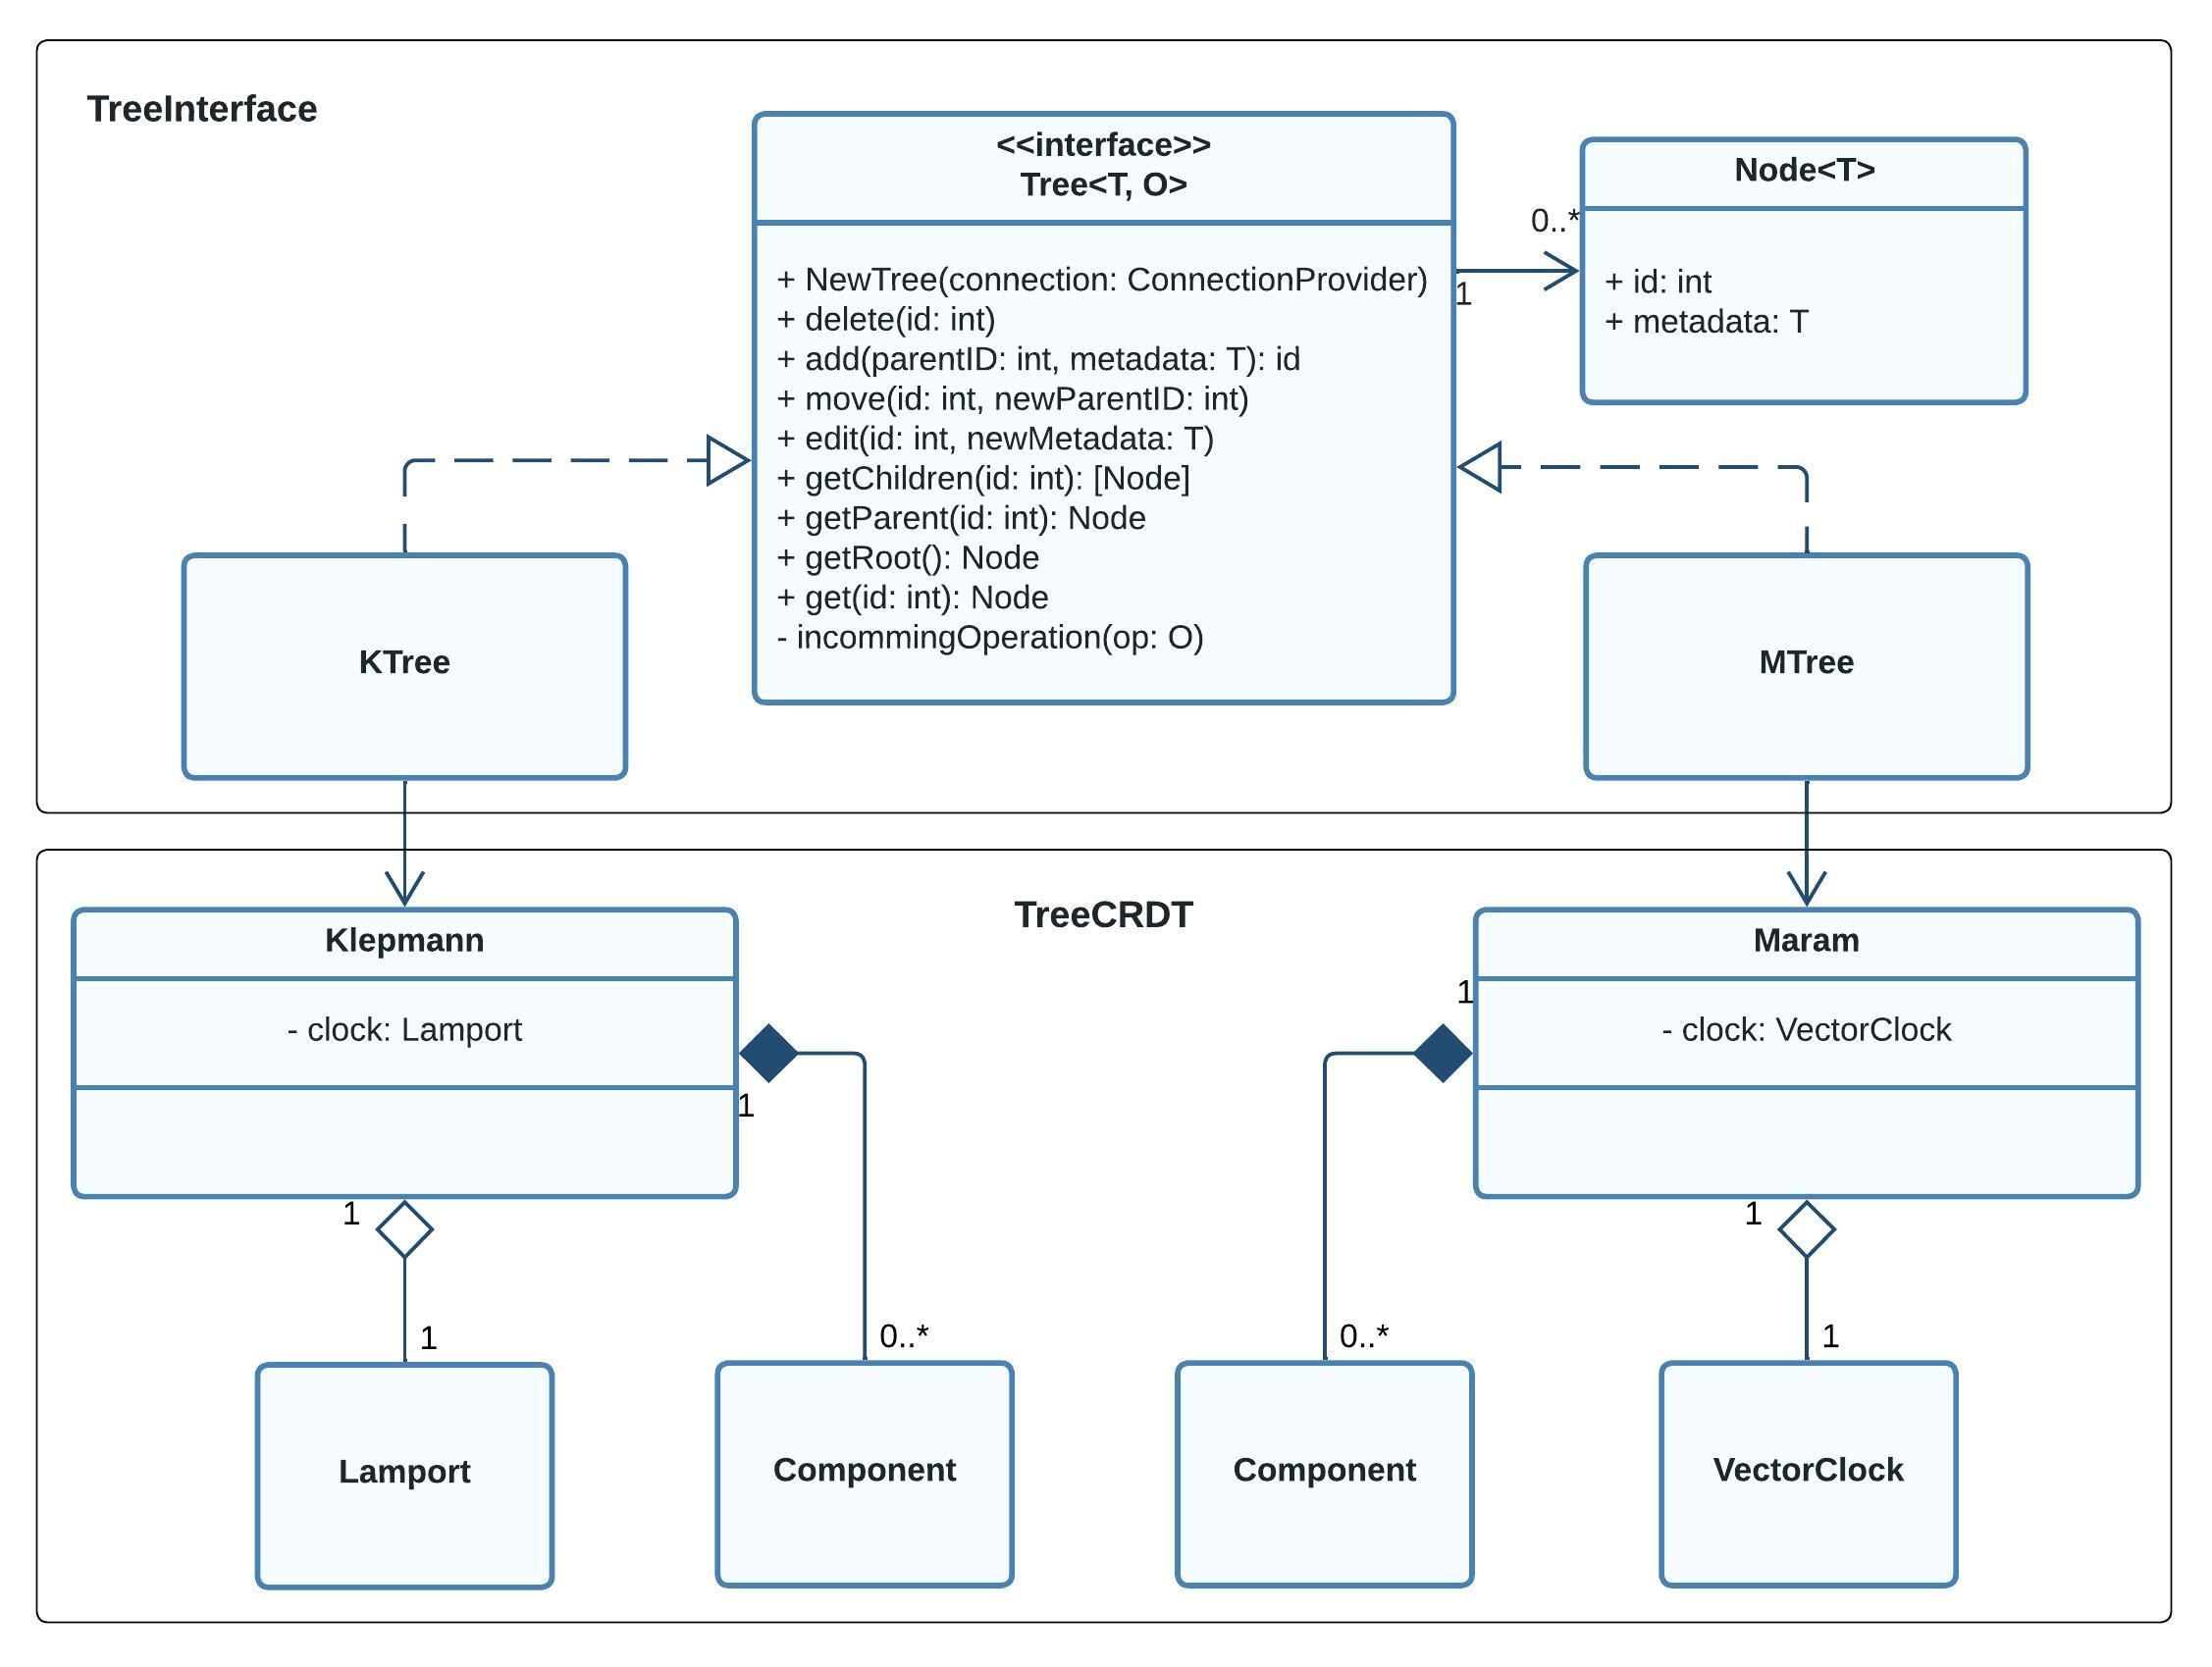
\includegraphics[width=13cm]{crdt.jpeg}}
    \caption{Class diagram for the CRDT and Interface layer. The \texttt{Tree} interface provides an interface for application code. Classes \texttt{MTree} and \texttt{KTree} provide implementations for the specific CRDTs.}
    \label{fig:crdt}
\end{figure}

\subsection{Network}
The network layer takes inspiration from Yjs\footnote{https://docs.yjs.dev/}, however the implementation is somewhat reversed. In Yjs, the network layer binds to the CRDT, in this paper the interface layer binds to the network layer. The main reason for this is that this paper is designing a static system, with a fixed number of nodes and therefore this design is more suitable. \par

If the system was to be designed to be dynamic, then the CRDT layer would have more requirements. The CRDT would either need to store all local operations indefinitely or provide a means of transferring its state to new nodes, as they would require access to the current state of the CRDT.

The network layer assumes that each node will be started with the same number of peers, and the total set of peers will not change. This is a reasonable assumption for a static system, however it is not suitable for a dynamic system. \par

\begin{figure}[h]
    \centering
    \fbox{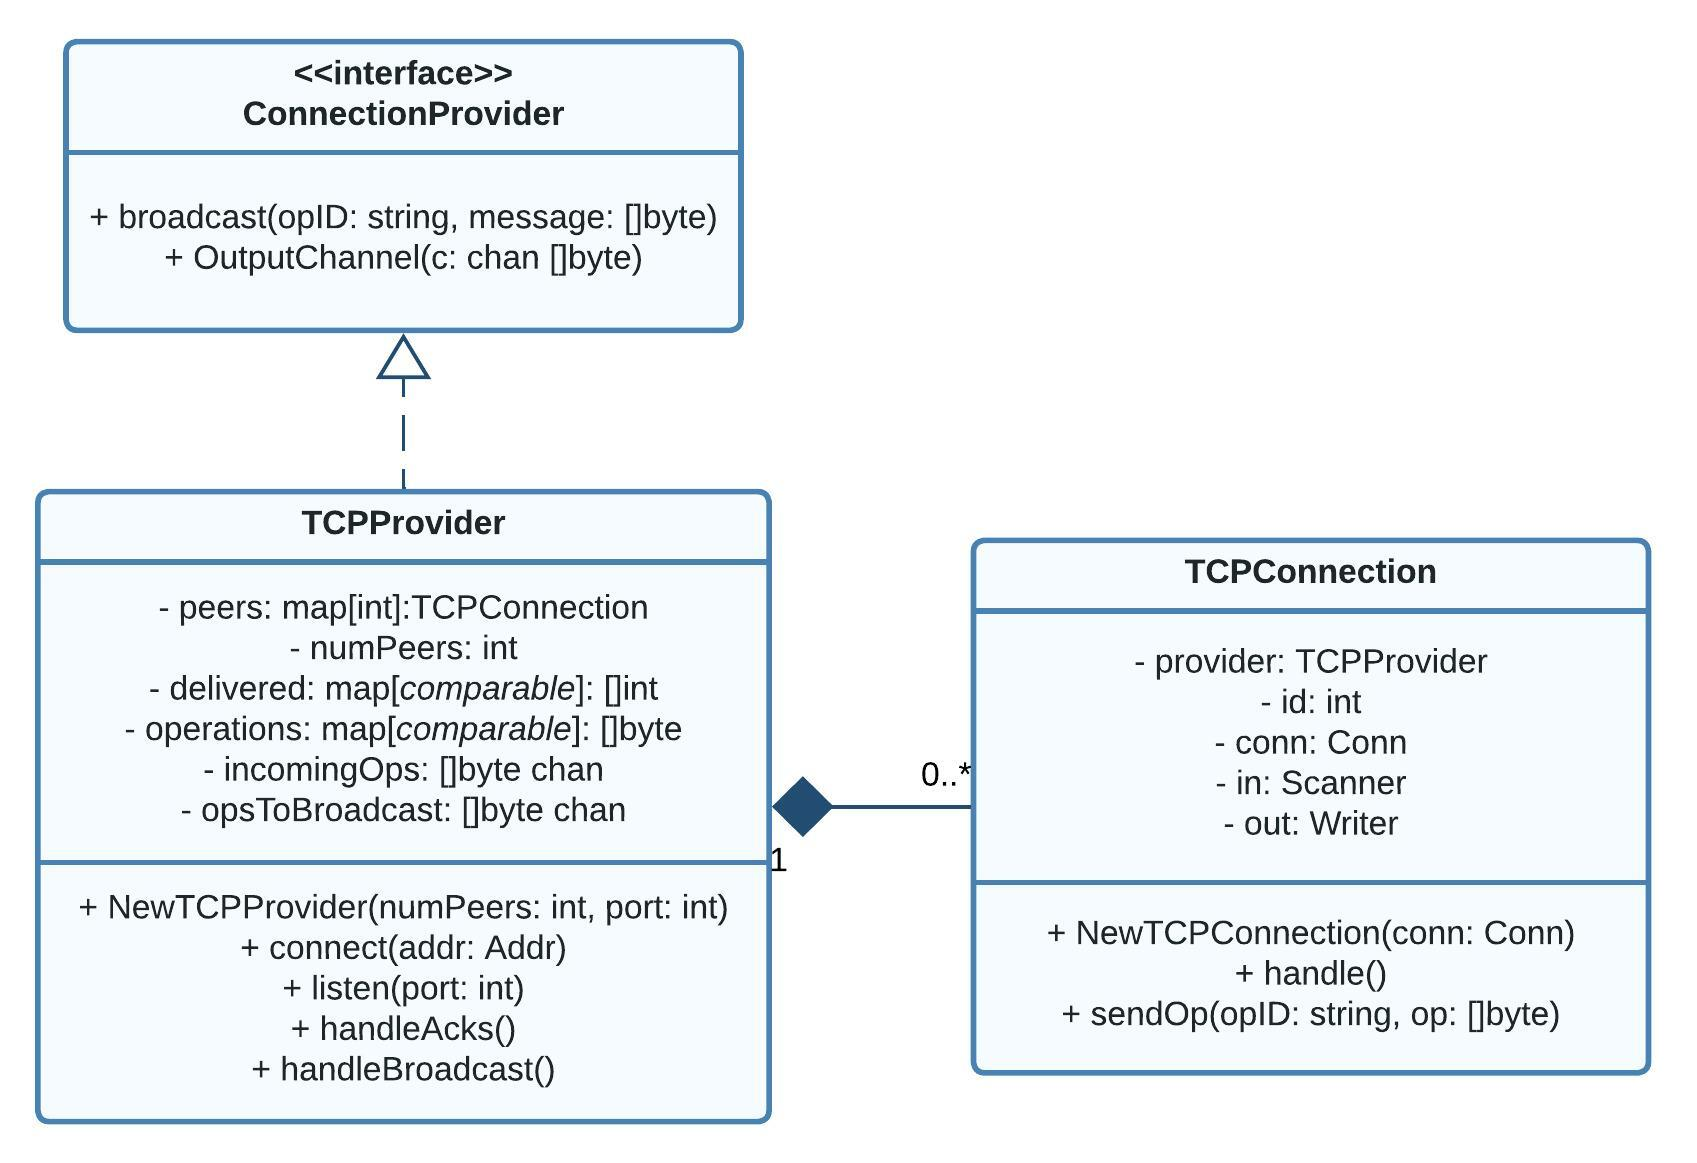
\includegraphics[width=12cm]{networkuml.jpeg}}
    \caption{Class diagram for the Network layer. With the interface \texttt{ConnectionProvider} and implementing class \texttt{TCPProvider}.}
    \label{fig:connection}
\end{figure}

The interface \texttt{ConnectionProvider} is shown in Figure \ref{fig:connection}. It describes what the network layer is required to do, broadcast messages and receive them. This interface is implemented by the class \texttt{TCPProvider}. The \texttt{TCPProvider} class is responsible for providing the reliable broadcast functionality, as well as listening for incoming connections. \par


The \texttt{TCPConnection} class is responsible for maintaining a connection with a single node, and receiving messages from that node. When a node joins after being offline, \texttt{TCPProvider} is responsible for sending them all the messages which they missed. The \texttt{TCPConnection} will not apply incoming operations, instead they will be passed to the TreeInterface for processing. This is useful as it reduces the need for locks, which would be required if the \texttt{TCPConnection} was responsible for applying operations. \par 

\section{Communication Sequences}
The CRDT layer and Clocks in the application should not be affected by concurrency because they are designed to be used in a single thread. Therefore, it is the responsibility of the developer to ensure that both are used exclusively within a single thread. The Interface and Network layer however will run in multiple threads, and therefore concurrency and message passing must be considered. \par

\subsection{Network Layer}

\begin{figure}[h]
    \centering
    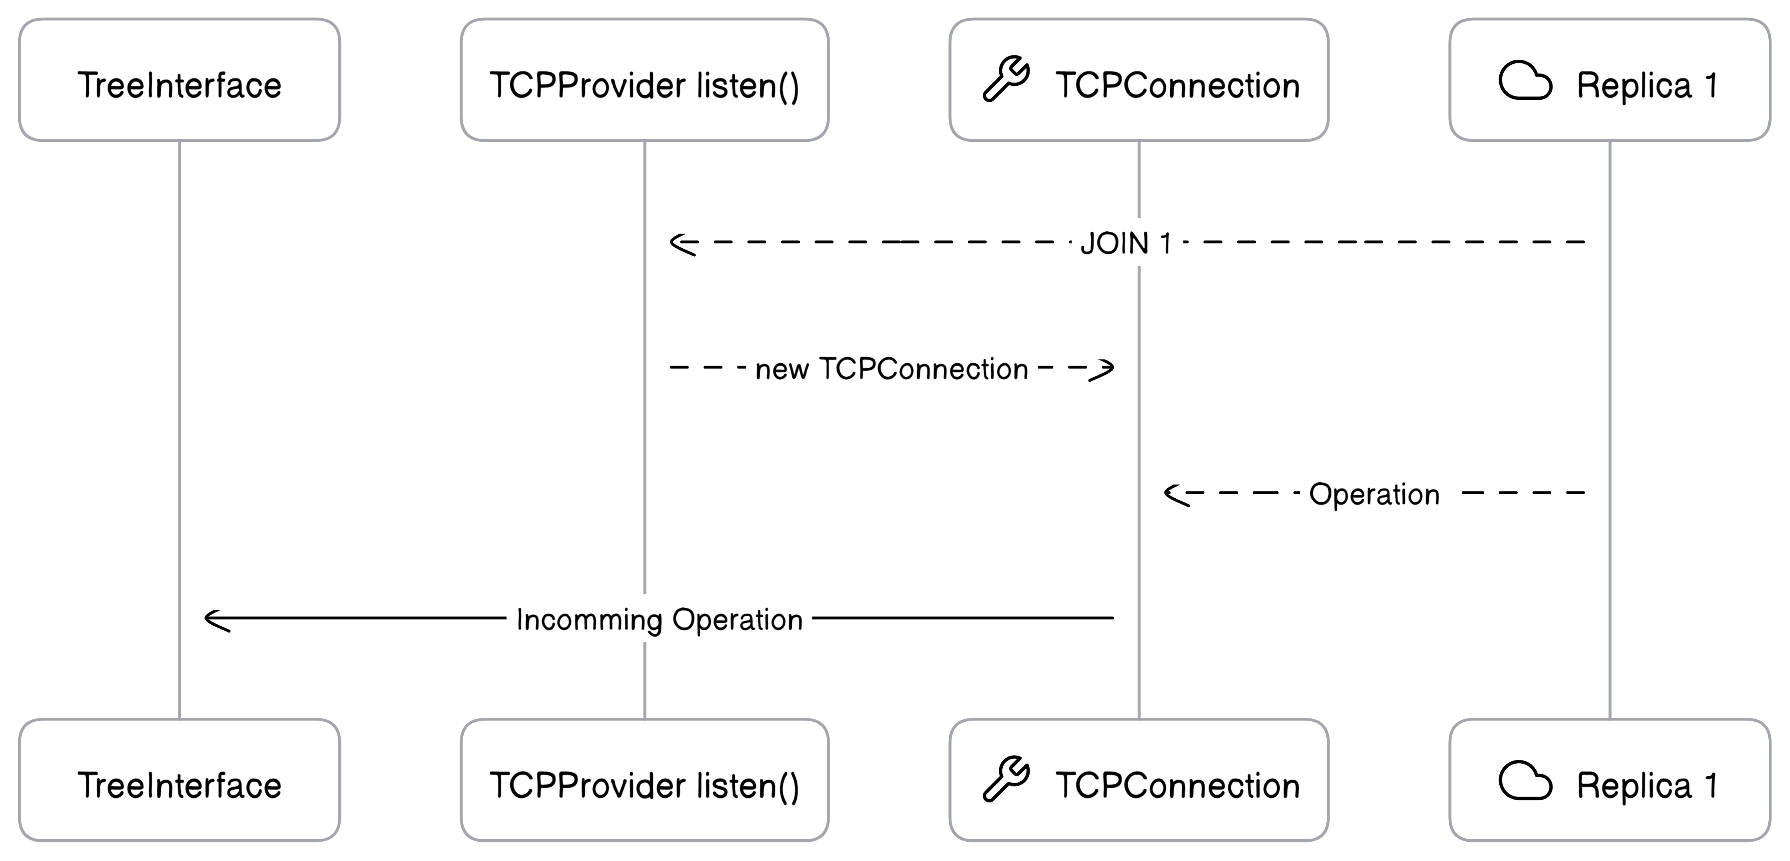
\includegraphics[width=1\textwidth]{networkjoin.png}
    \caption{Sequence diagram for the network layer, showing a replica connecting and sending an operation.}
    \label{fig:networkjoin}
\end{figure} 

\begin{figure}[h]
    \centering
    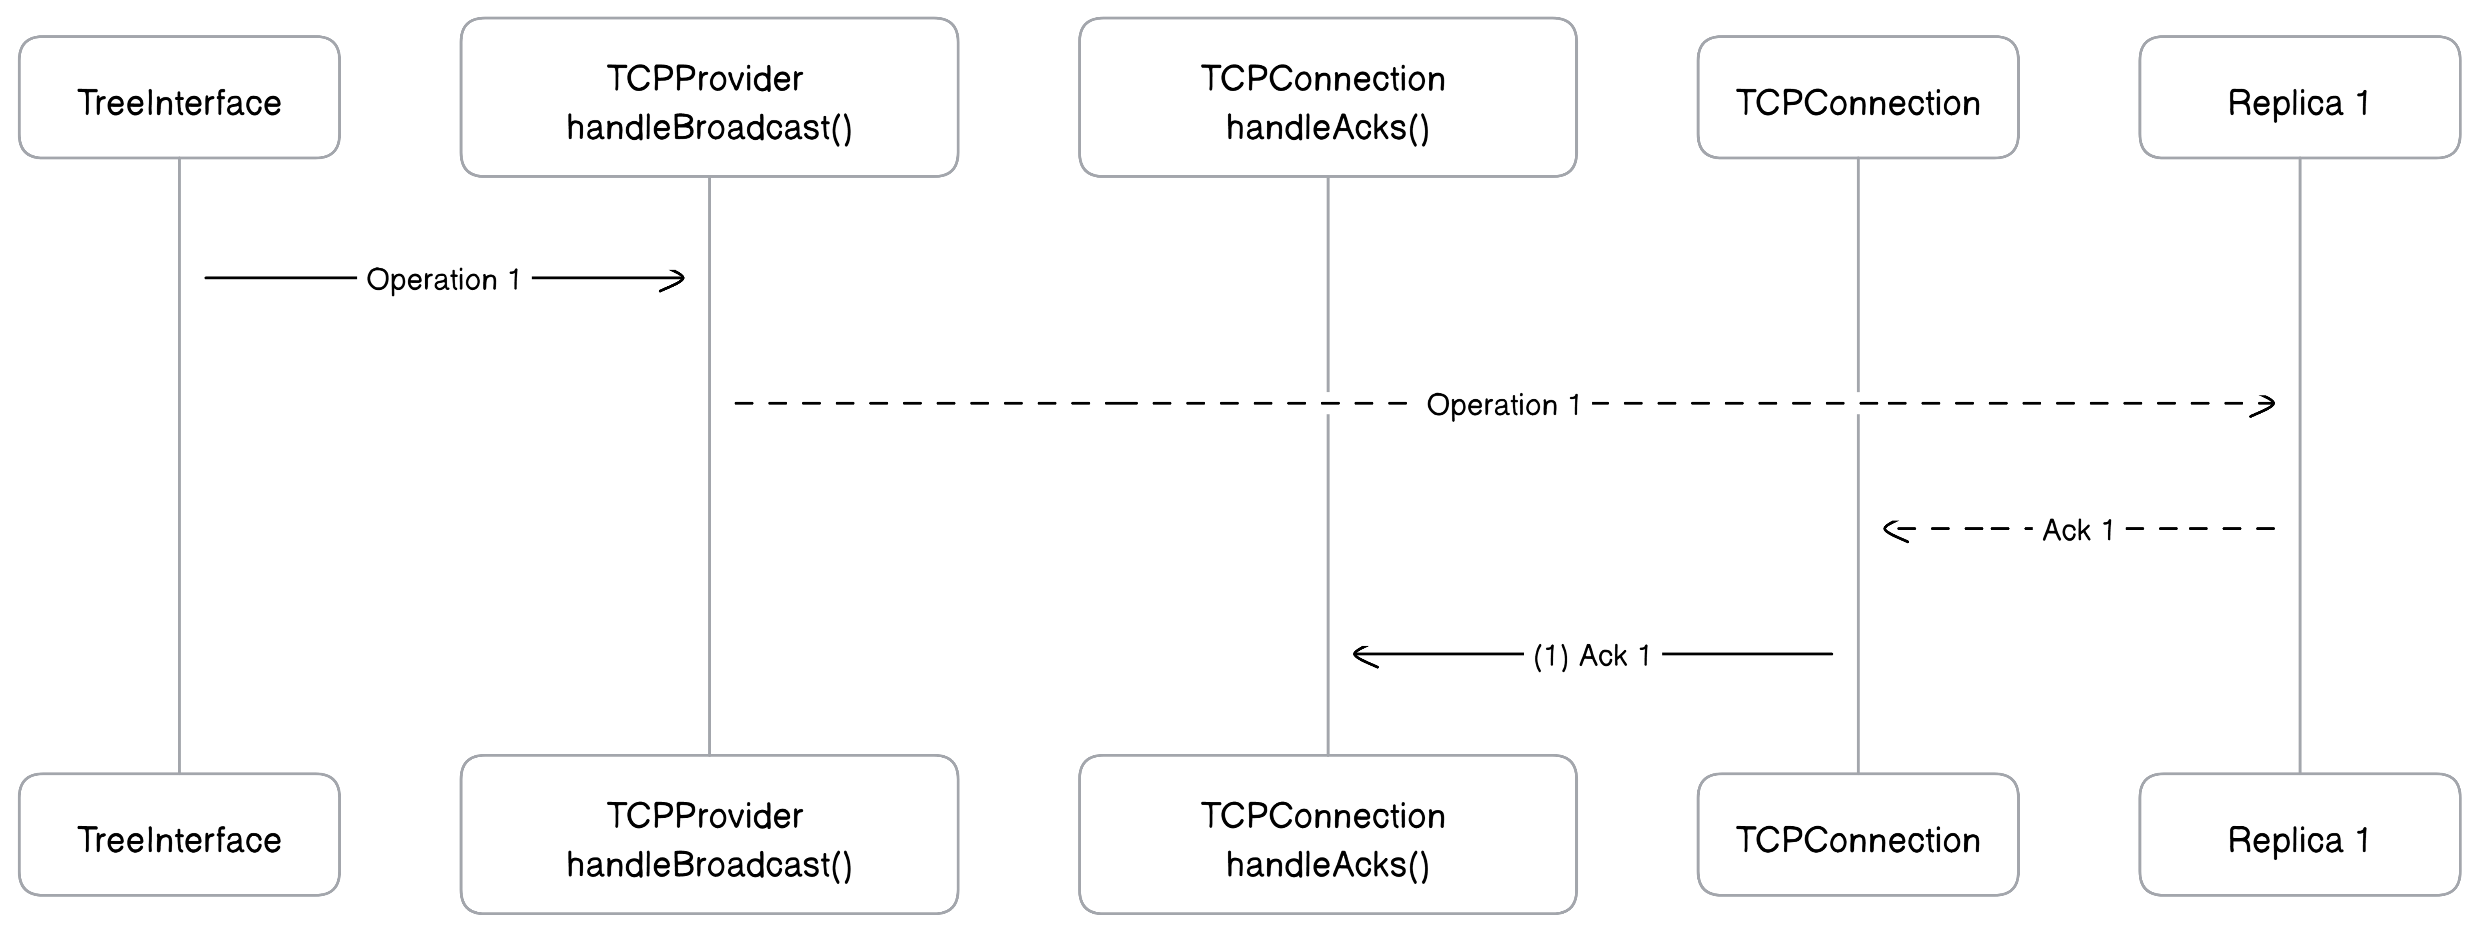
\includegraphics[width=1\textwidth]{networksend.png}
    \caption{Sequence diagram for the network layer, showing an operation being sent and an acknowledgement being received.}
    \label{fig:networksend}
\end{figure} 

The network layer will comprise multiple concurrent processes. One process will be responsible for listening for incoming connections, and creating a new \texttt{TCPConnection} for each connection. The \texttt{TCPConnection} will only be responsible for receiving messages from the peer but not sending them. If the message is an operation, it is sent to the TreeInterface buffer to be applied to the Tree. Otherwise, if it is an acknowledgement, it is sent to \texttt{TCPProvider handleAcks()} for processing. As show by Figure \ref{fig:networkjoin} and \ref{fig:networksend}. \par

The \texttt{TCPProvider} will be responsible for sending messages to other peers, which will happen in a separate process as show by Figure \ref{fig:networksend}. The process will receive operations to send from the Interface layer. Whenever an operation is broadcasted, it is added to a map that associates the operation's ID with a list of node IDs. When a node sends an acknowledgement for an operation, that node ID is added to the list of node IDs for that operation. When the list of node IDs is the same size as the number of nodes, the operation is removed from the map. This is how the system ensures each node receives each operation. \par



\subsection{Interface Layer}

As shown by Figure \ref{fig:interfaceseq}, the interface layer will buffer operations from the network layer, and only apply them when they are ready. This is important for the causal consistency model, as it ensures that operations are applied in the correct order. For local operations, they are translated into operations for the specific CRDT, and then applied to the CRDT. It is likely that the CRDT will be protected by a lock, as it is not thread safe. \par

Broadcasting operations is not shown in Figure \ref{fig:interfaceseq}, but it would happen after the operation is applied to the CRDT. A message would be sent to the network layer, which would then broadcast the operation to all other nodes. \par

\begin{figure}[h]
    \centering
    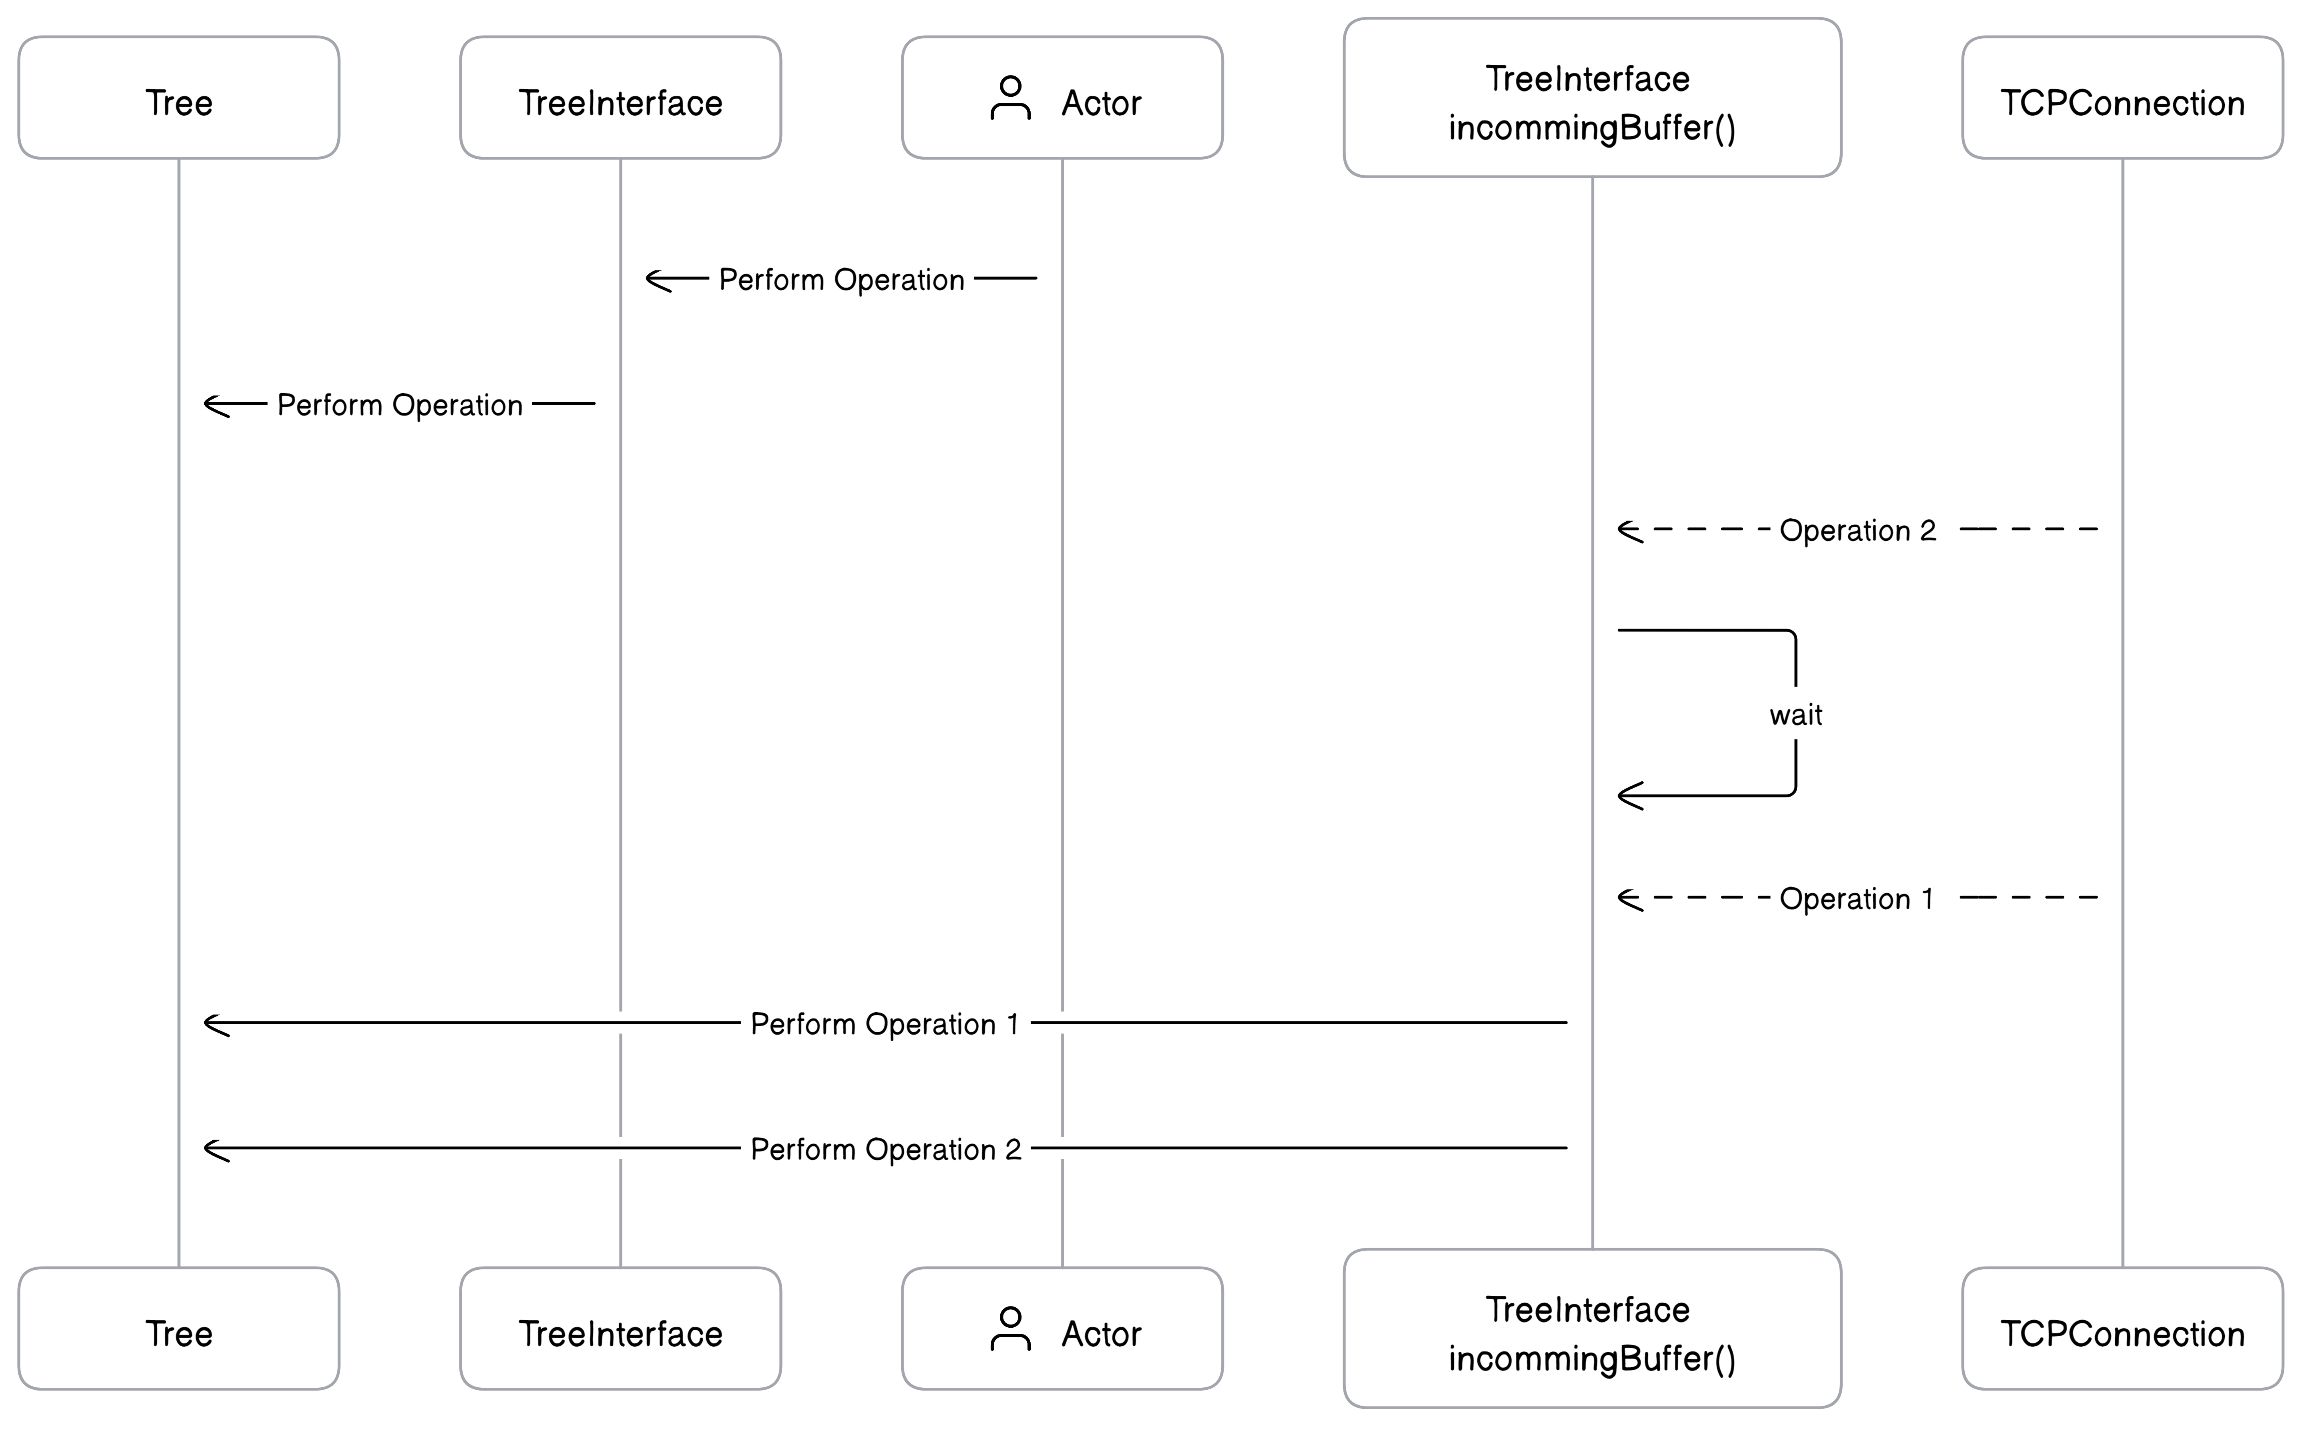
\includegraphics[width=1\textwidth]{treeinterface.png}
    \caption{Sequence diagram for the interface layer, showing operations being applied to the Tree. Broadcasting is not shown.}
    \label{fig:interfaceseq}
\end{figure}


\section{Justification of Design}
The design is split into four packages, which helps to keep the code modular and easy to understand. Each package has a single responsibility, which helps to keep the code easy to maintain. This design approach of having a single responsibility for each package and having interdependencies between packages is a common design pattern in software engineering. \par

The system takes advantage of concurrency to allow for increased performance and scalability. Message passing will be used to reduce the need for locks, which can otherwise cause performance issues. The use of multiple threads also allows for the system to be more responsive, as it can handle multiple requests at once. Each thread will be responsible for a single task, which will help to keep the code easy to understand. \par


\chapter{Implementation}\label{sec:implementation}

\chapter{Testing}

\chapter{Evaluation}

%TC:ignore
\addcontentsline{toc}{chapter}{References}
\printbibliography

\appendix

\chapter{Interim Project Management}

\section{Account of Work to date}
The current work has been around reviewing relevant literature and creating an initial design from this research. The research has been into current systems for file synchronisation, and their drawbacks. As well as into distributed systems and consistency models. Most importantly, detailed research has been completed into CRDTs and ones applicable to this paper's proposed system. From this research, an initial design has been created outlining the main aspects of the proposed system.

\section{Plan of remaining work}
The design will be refined and more detailed. From this design, the CRDT layer will be implemented by first selecting an algorithm and then coding it. Then, the Network layer, where the peer-to-peer networking will be coded first, followed by operation transmission and finally file data transmission. Then, the File System layer, where the watcher (which watches the file system for changes) will be coded and then reading and writing file content. Development of these layers may overlap, but it will follow the general structure listed. \par
Once all components have been coded, the system will have its reliability and performance tested, which will inform the evaluation. The testing will seek to measure the throughput and response time of the algorithm(s), and how adding more replicas affects this. The evaluation then needs to be written and will contain the outcome of the project.

\section{Estimate of Support Required}
The performance testing may require the use of rented servers, to test latency.

\section{Gantt Chart}

\subsection{Completed Work}
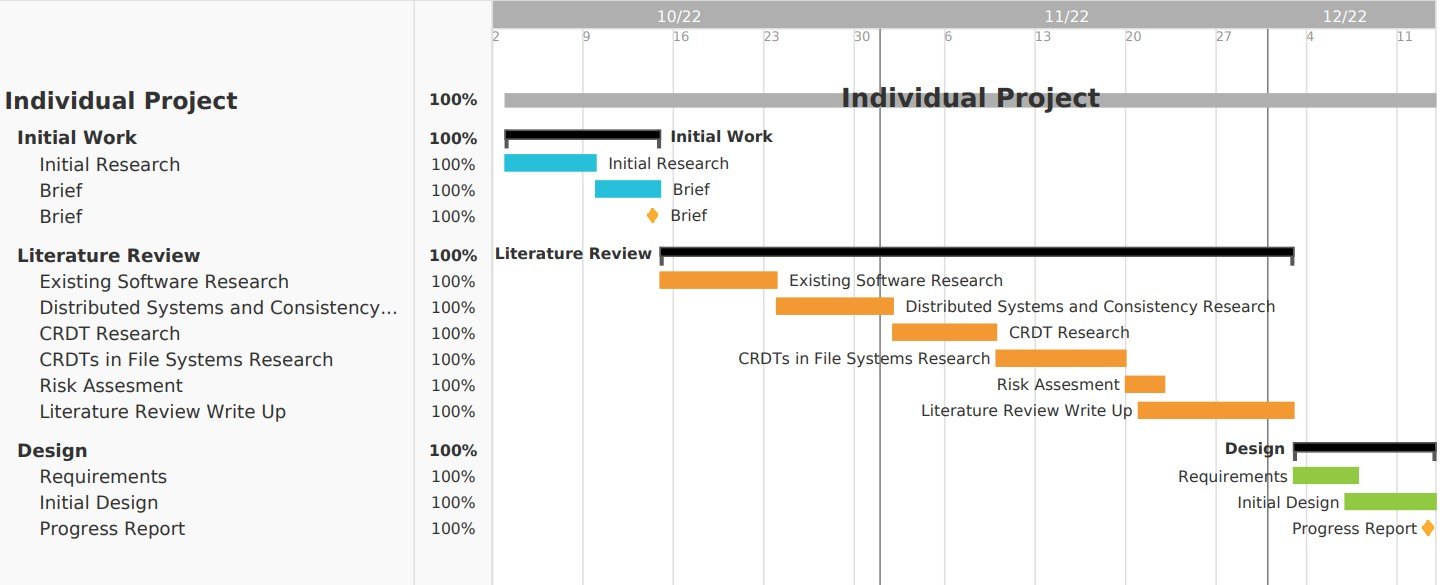
\includegraphics[width=16cm]{completed.jpg}


\subsection{Remaining Work}
\begin{center}
    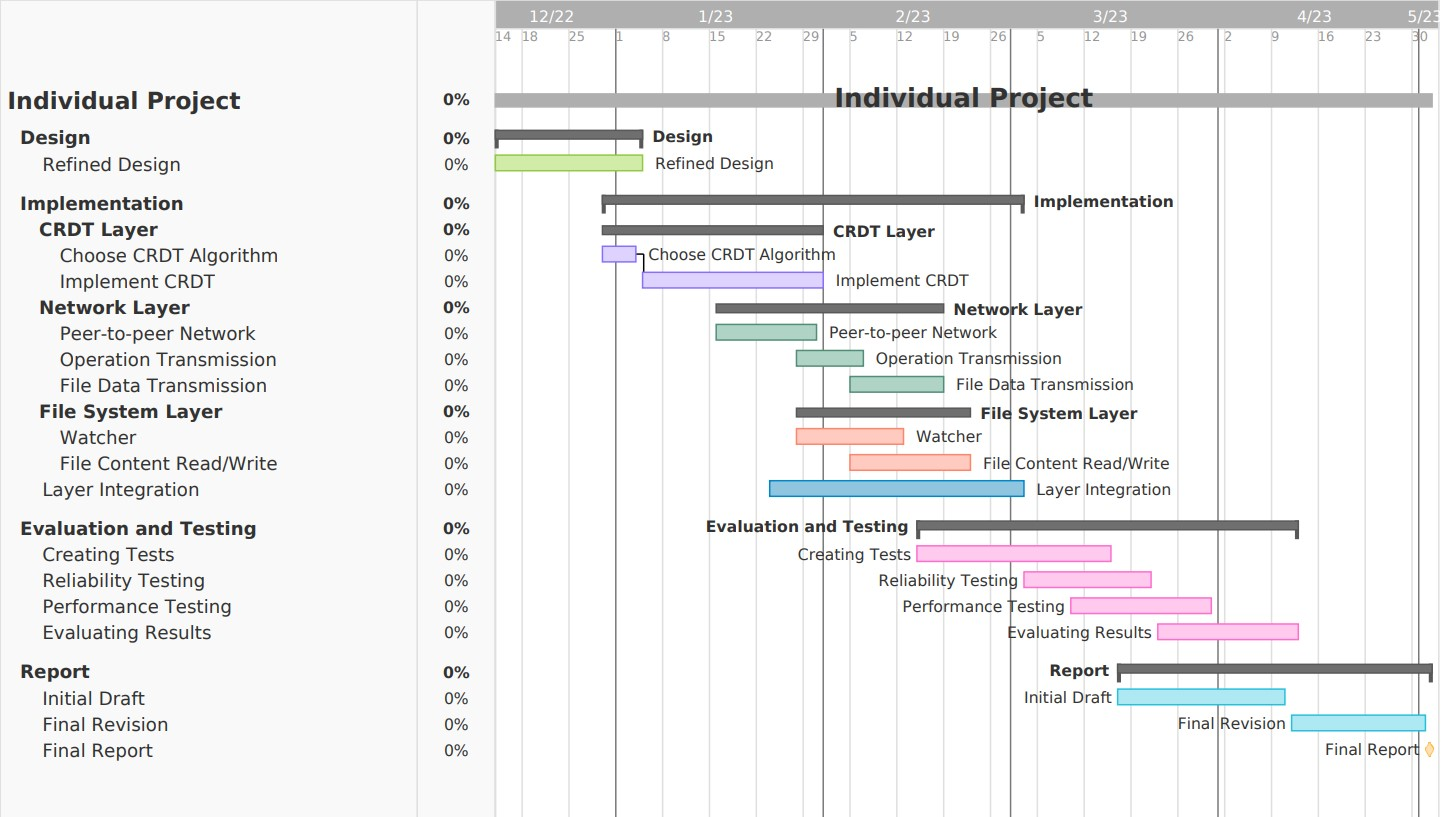
\includegraphics[width=16cm]{remaining.jpg}
\end{center}


\section{Risk Assessment}

\begin{itemize}
    \item \textbf{(P) Probability} 1 - low, 5 - high
    \item \textbf{(S) Severity}  1 - low, 5 - high
    \item \textbf{(RE) Risk Exposure} Probability * Severity
\end{itemize}

\begin{table}[htbp]
    \renewcommand{\arraystretch}{1.3}
    \captionsetup{
        font=normalsize,
        skip=2pt % adjust the value as needed
    }
    \caption{Risk Assessment} % title of Table 
    \centering % used for centering table
    \begin{tabular}{|p{3cm} | p{0.4cm} | p{0.4cm} | p{0.6cm} | p{8cm}|} % centered columns (4 columns)
        \hline\hline %inserts double horizontal lines
        \textbf{Risk}               & \textbf{P} & \textbf{S} & \textbf{RE} & \textbf{Mitigation}                                                                                              \\ [0.5ex] % inserts table
        %heading
        \hline % inserts single horizontal line
        Loss of Report             & 2          & 5          & 10          & Back-up on computer, laptop and OneDrive                                                                         \\ \hline % inserting body of the table
        Loss of Code                & 1          & 5          & 5           & Back-up on computer, laptop, OneDrive and GitHub                                                                 \\ \hline
        Underestimating Tasks       & 3          & 3          & 9           & Plan for extra time in case tasks require it, as well as making informed estimates for time needed for each task \\ \hline
        Health Issues               & 2          & 4          & 8           & Allow for spare time, and possible removal of parts of project. Attempt to not become sick.                      \\ \hline
        Implementation Difficulties & 3          & 4          & 12          & Create a clear plan of work to do, and take time to understand the design. Can seek help if needed.              \\ \hline
        Change in Scope             & 2          & 4          & 8           & Complete implementation early to allow for changes to the scope.
        \\ \hline %inserts single line
    \end{tabular}
    \label{table:risk} % is used to refer this table in the text
\end{table}

\chapter{Original Brief}
\section{Original Title}
\begin{center}
Using CRDTs to Create a File Synchronization System
\end{center}

\section{Problem}
Distributed computing systems are becoming more popular for two main reasons, availability
and scalability. Distributed storage systems that have replicas need a way to merge the replicas,
however conflicts can arise when merging two different replicas. Software such as Google Drive
and Dropbox exhibit bugs in their concurrency control when the filesystem is concurrently
updated on different computers. CRDTs (Conflict-free Replicated Data Types) can be
implemented to ensure strong eventual consistency (SEC) as well as remove the need for a
centralized server or leader. SEC ensures that two nodes/peers will converge to the same state
even if the order in which they receive a set of updates is different. CRDTs can have the benefit
of a low-latency because updates can be made locally without having to contact another node,
however their throughput may be lower than other solutions, such as state machines, due to
them having to resolve conflicts. Due to the high guarantees of CRDTs, implementations for
complex data types are still being theorized and tested in practice (such as tree CRDTs).

\section{Goal} 
The goal of this project is to implement and test the performance and viability of using new
advancements in tree CRDTs in a file synchronization system to solve directory conflicts. This
project aims to be able to demonstrate whether using CRDTs in this application is viable, mainly
focusing on the throughput and reliability of the system. The system should be able to tolerate
network failures and offline usage. The implementation will be peer-to-peer, meaning that each
node will be equally privileged. Another focus of this project will be on optimisation and so
different methods will be documented to show how this was achieved, with a focus on
increasing throughput (as CRDTs have naturally low latency).
Tree structures are used in many scenarios so the code for this project could be used in other
scenarios when Strong Eventual Consistency is wanted.

\section{Scope}
The scope of this project will be limited to implementing CRDTs to resolve directory conflicts and
testing their performance and reliability. The system should be tested with a varying number of
replicas to attempt to visualize how the system would scale. Optimisations will only be
implemented after the system works as intended.
File conflicts will not be a focus of this project, however they could be brought into the scope if
time allows.

\section{Interim Abstract}
This report is an attempt to use new developments in tree CRDTs with
highly available move operations to create a file synchronisation system that
will resolve all directory conflicts without human interaction; and will not
exhibit ’buggy’ behaviour such as duplicating files which some current systems exhibit. This report should provide research into the viability of these
systems in a real-world scenario. So far, this paper has reviewed the existing
literature and has analysed the concurrency issues facing current systems. As
well as detailing two algorithms which have been proposed that state to have
solutions to the problem of creating a highly available move operation.
The remaining work includes creating a more refined design of the system and
then implementing the separate parts to create a cohesive application. Once
implemented, the system will be tested for reliability and performance. This
testing will inform the final evaluation of system, where it will be compared
to existing solutions.


%TC:endignore
\end{document}

